I% Chapter Template

\chapter{Performance} % Main chapter title

\label{Performance} % Change X to a consecutive number; for referencing this chapter elsewhere, use \ref{ChapterX}

\lhead{Performance. \emph{Performance in practice and Benchmarks}} % Change X to a consecutive number; this is for the header on each page - perhaps a shortened title


%----------------------------------------------------------------------------------------
%	SECTION In practice: Running on JVM
%----------------------------------------------------------------------------------------
\section{In practice: Running on JVM}
% code interpreted vs compiled
% GC and memory allocations
% system arraycopy primitive

%-----------------------------------
%	SUBSECTION Cost of Abstraction
%-----------------------------------
\subsection{Cost of Abstraction and JIT Inline}
% cost of function invokation
% code compiled (inlined if hot)
% aim to make all critical methods 35< bytes


%----------------------------------------------------------------------------------------
%	SECTION Scalameter
%----------------------------------------------------------------------------------------
\section{Measuring performance}
% Scalameter
% warmup to JIT inline
% using vectors that do not fill perfectly the last branch to avoid trivial cases (that would be faster but do not show the average of the operation)


%----------------------------------------------------------------------------------------
%	SECTION Generators
%----------------------------------------------------------------------------------------
\section{Generators}
% block sizes
% concat implementation
% balanced, a bit unbalanced and extremely unbalanced



%----------------------------------------------------------------------------------------
%	SECTION Benchmarks
%----------------------------------------------------------------------------------------
\section{Benchmarks}
% describe the the different benchmark types 
%% differences between implementation (vector vs rrbvector)
%% differences between unbalances
%% differences between block sizes
%% differences between concatenation rebalancing method

%-----------------------------------
%	SUBSECTION Apply
%-----------------------------------
\subsection{Apply}
% describe the benchmark function
% compare expectation with results
% explain the upper bound
% explain apparently incoherent results

\begin{figure}[h!]
  \centering
  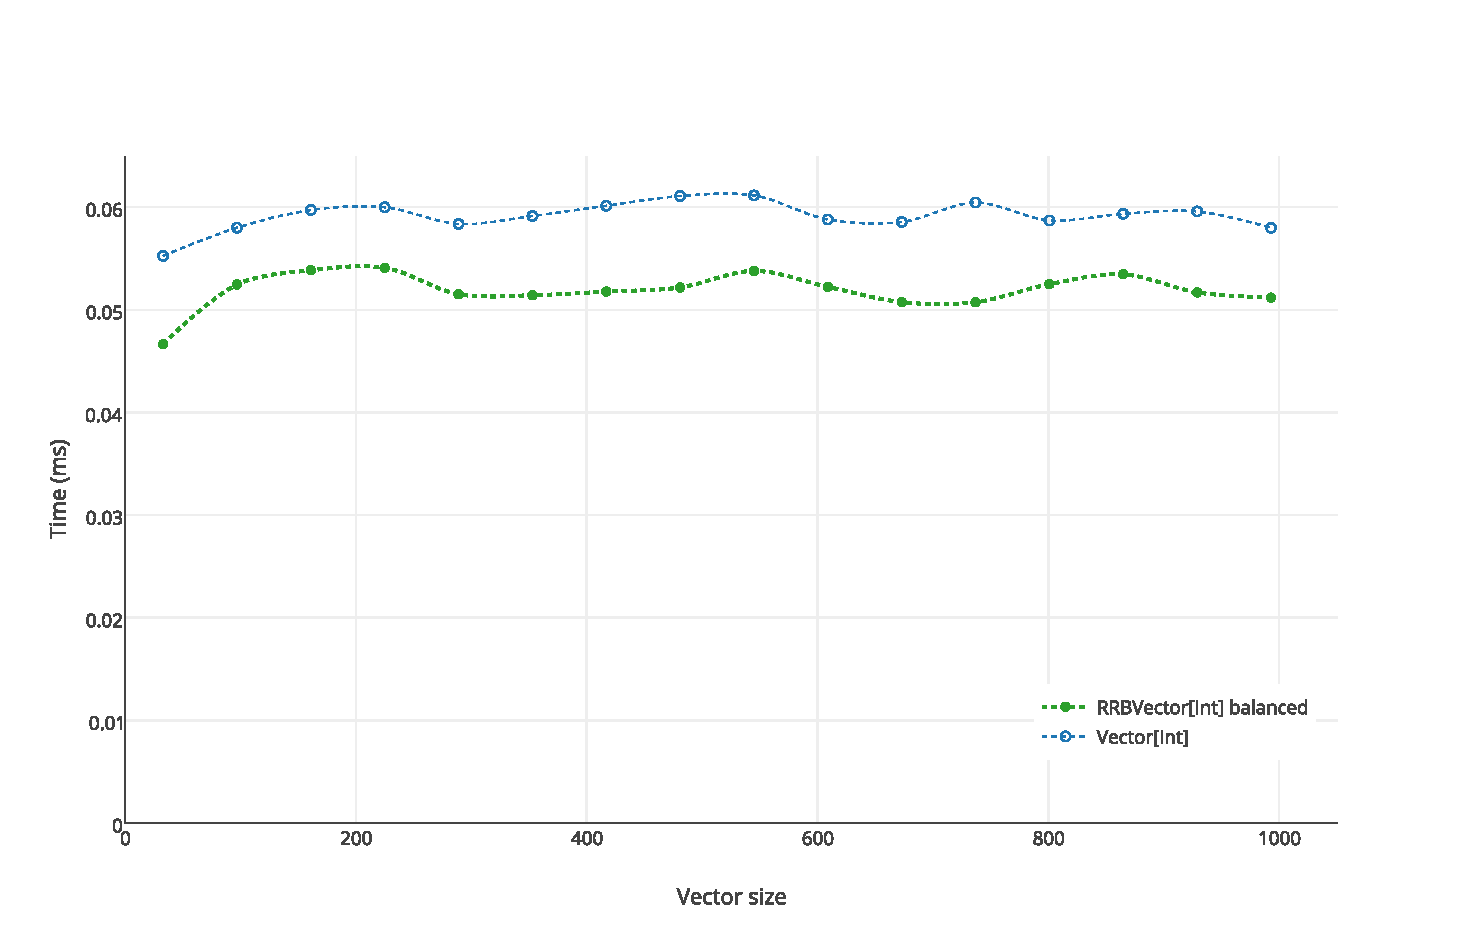
\includegraphics[width=\textwidth]{Benchmarks/Apply_2.pdf}
  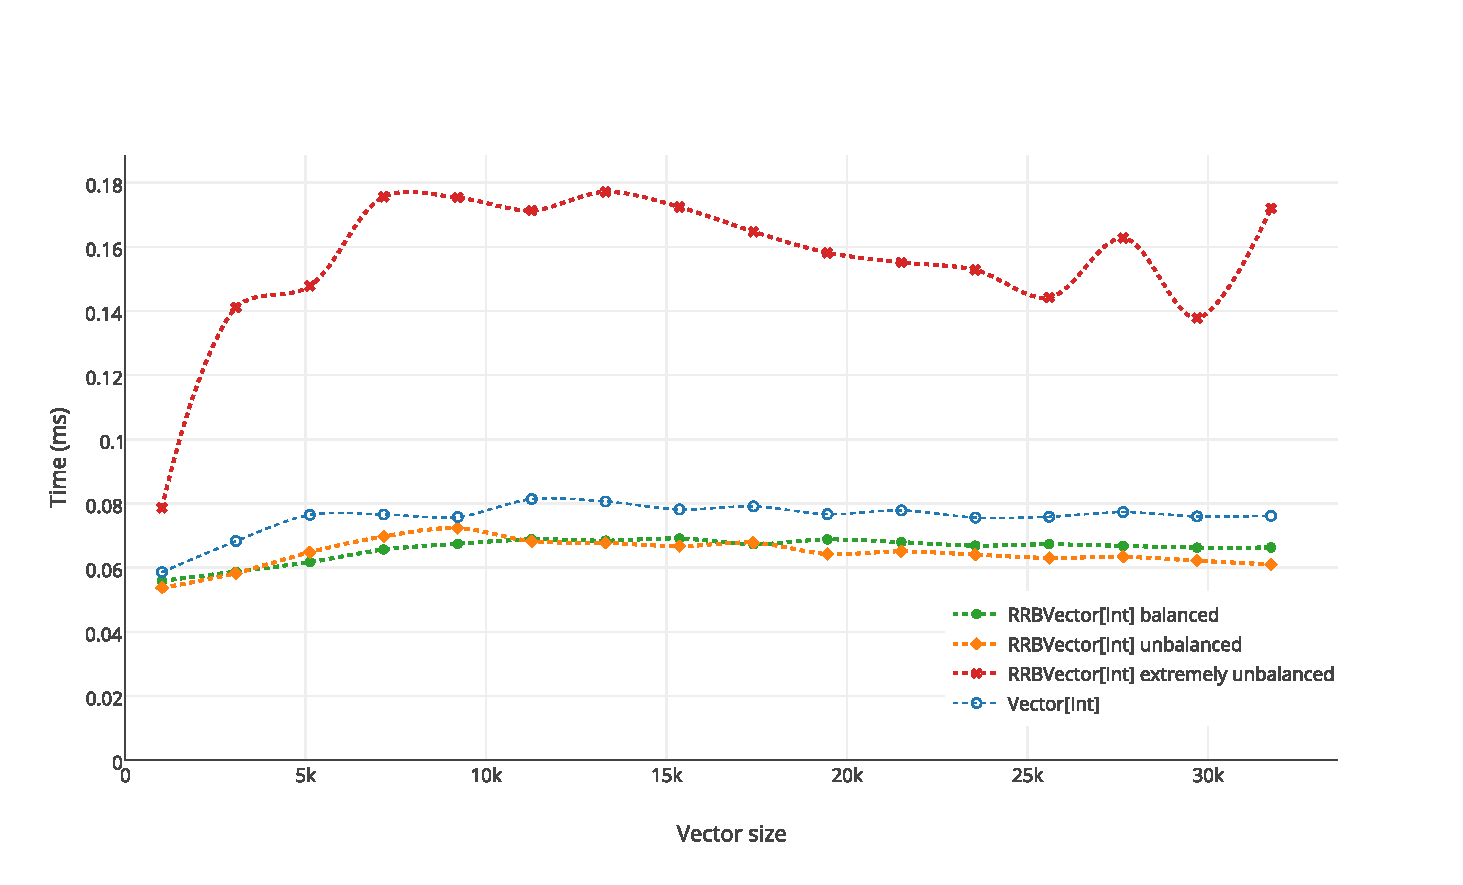
\includegraphics[width=\textwidth]{Benchmarks/Apply_3.pdf}
  \label{ApplyBenchmarks}
  \caption{Time to execute 10k apply operations on sequential indices.}
\end{figure}

\begin{figure}[h!]
  \centering
  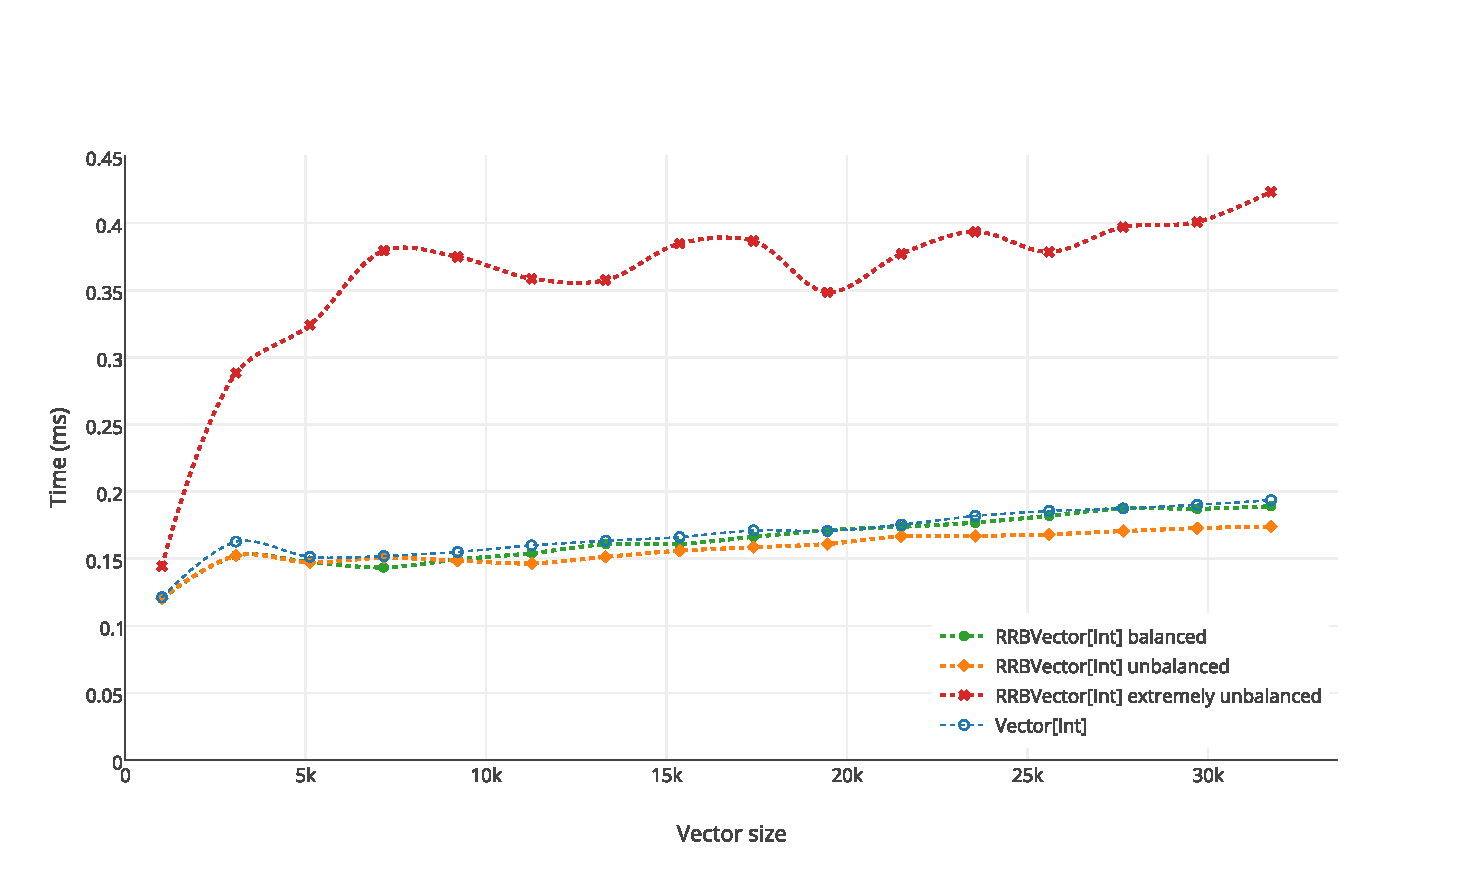
\includegraphics[width=\textwidth]{Benchmarks/Apply_random_3.pdf}
  \label{ApplyRandomBenchmarks}
  \caption{Time to execute 10k apply operations on random indices.}
\end{figure}

\begin{figure}[h!]
  \centering
  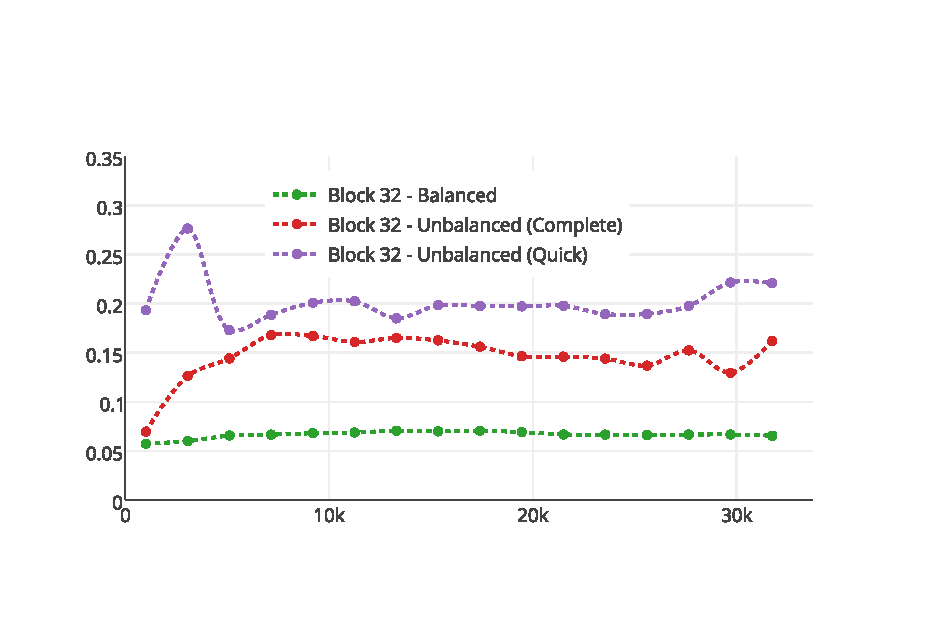
\includegraphics[width=0.49\textwidth]{Benchmarks/Apply_blocks_32.pdf}
  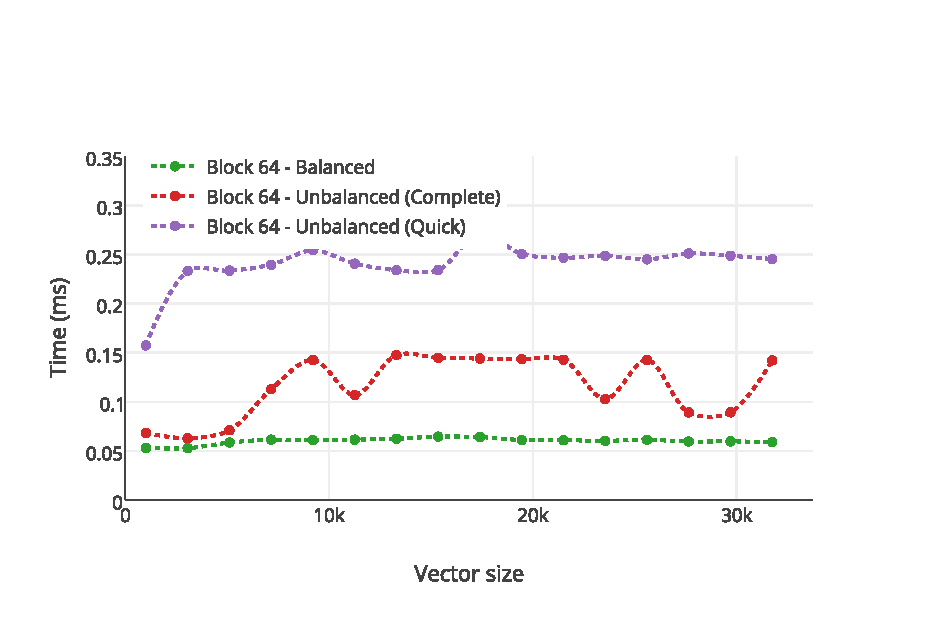
\includegraphics[width=0.49\textwidth]{Benchmarks/Apply_blocks_64.pdf}
  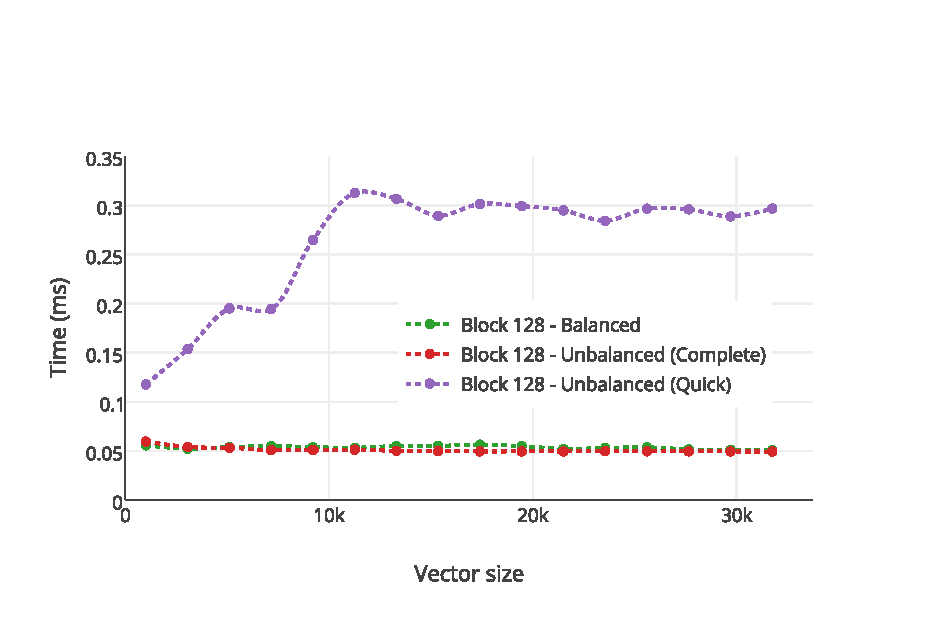
\includegraphics[width=0.49\textwidth]{Benchmarks/Apply_blocks_128.pdf}
  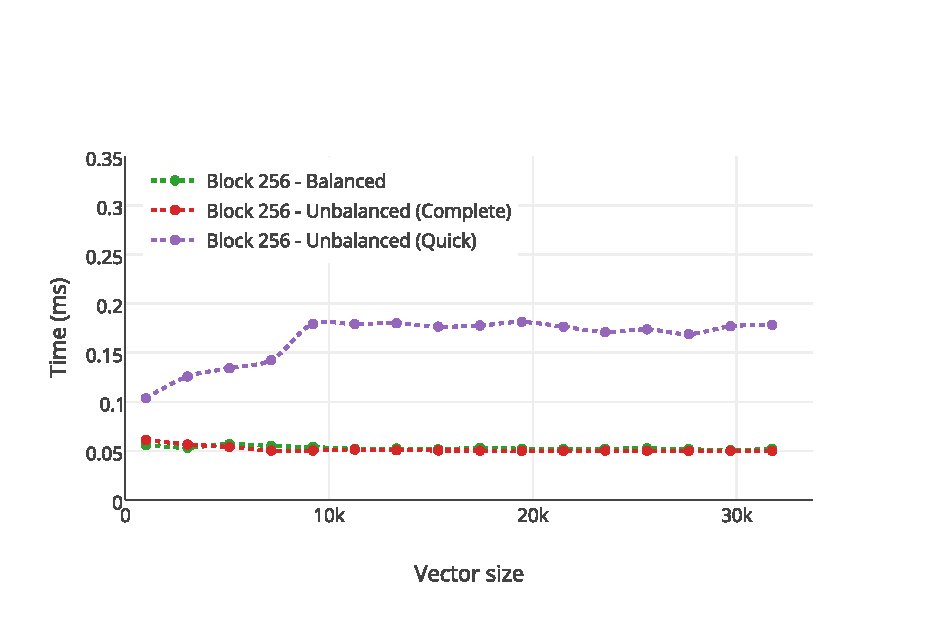
\includegraphics[width=0.49\textwidth]{Benchmarks/Apply_blocks_256.pdf}
  \label{ApplyBlocksBenchmarks}
  \caption{Time to execute 10k apply operations on sequential indices. Comparing performances for different block sizes and different implementation of the concatenation inner branch rebalancing (Complete/Quick).}
\end{figure}

%-----------------------------------
%	SUBSECTION Concatenation
%-----------------------------------
\subsection{Concatenation}
% describe the benchmark function
% compare expectation with results
% explain the upper bound
% explain apparently incoherent results

\begin{figure}[h!]
  \centering
  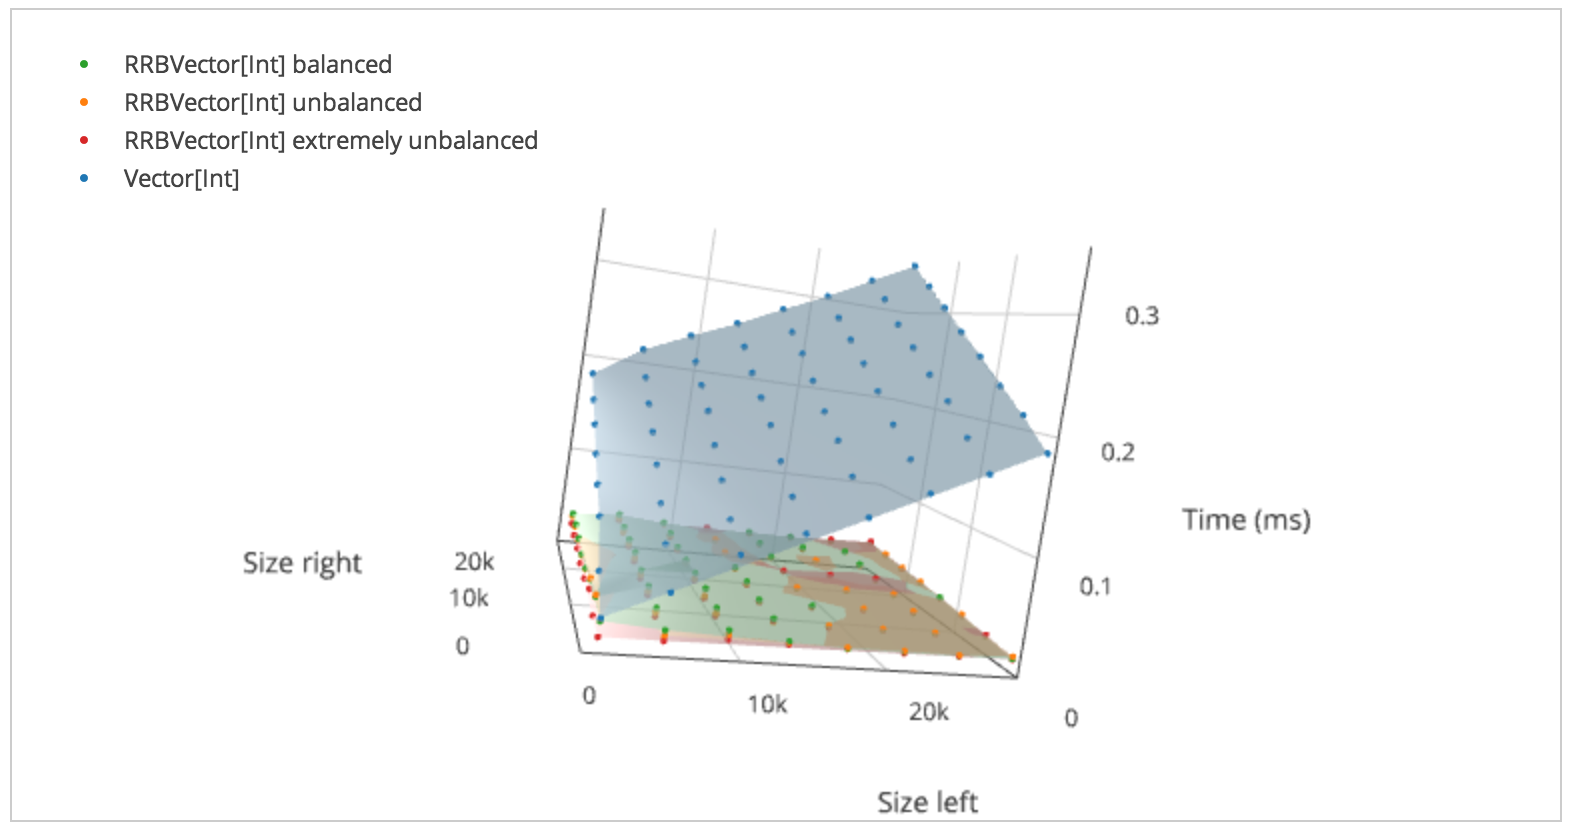
\includegraphics[width=\textwidth]{Benchmarks/Concat.png}
  \label{ConcatBenchmarks}
  \caption{Execution time for a concatenation operation on two vectors. In theory (and in practice) Vector concatenation is $O(left + right)$ and the rrbVector concatenation operation is $O(log_{32}(left + right))$.}
\end{figure}

%-----------------------------------
%	SUBSECTION Append
%-----------------------------------
\subsection{Append}
% describe the benchmark function
% compare expectation with results
% explain the upper bound
% explain apparently incoherent results

\begin{figure}[h!]
  \centering
  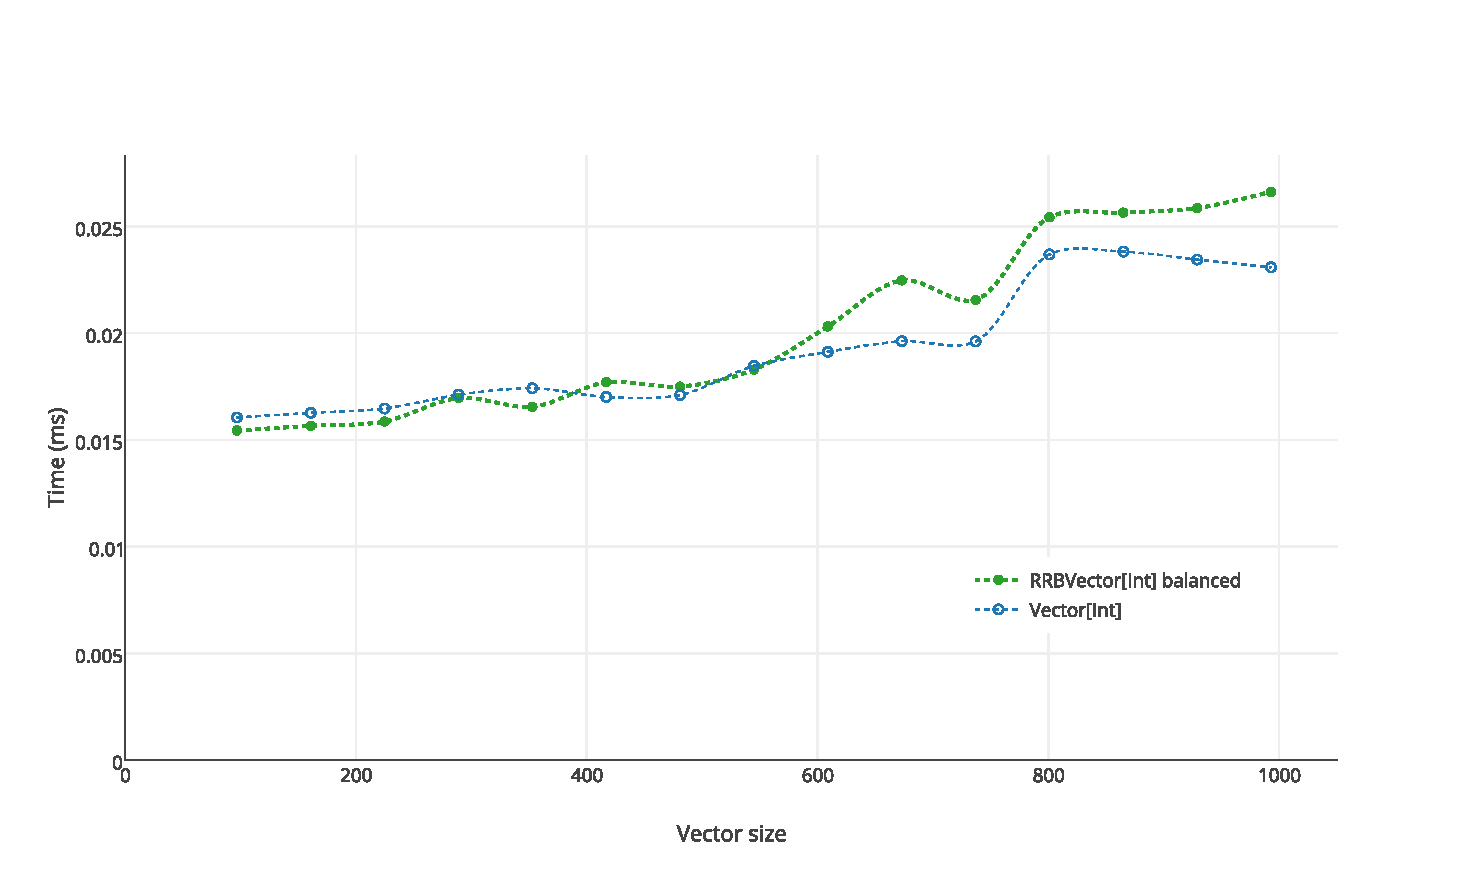
\includegraphics[width=\textwidth]{Benchmarks/Append_2.pdf}
  \label{Append2Benchmarks}
  \caption{Time to execute 256 append operations. This shows the amortized cost of the append operation.}
\end{figure}

\begin{figure}[h!]
  \centering
  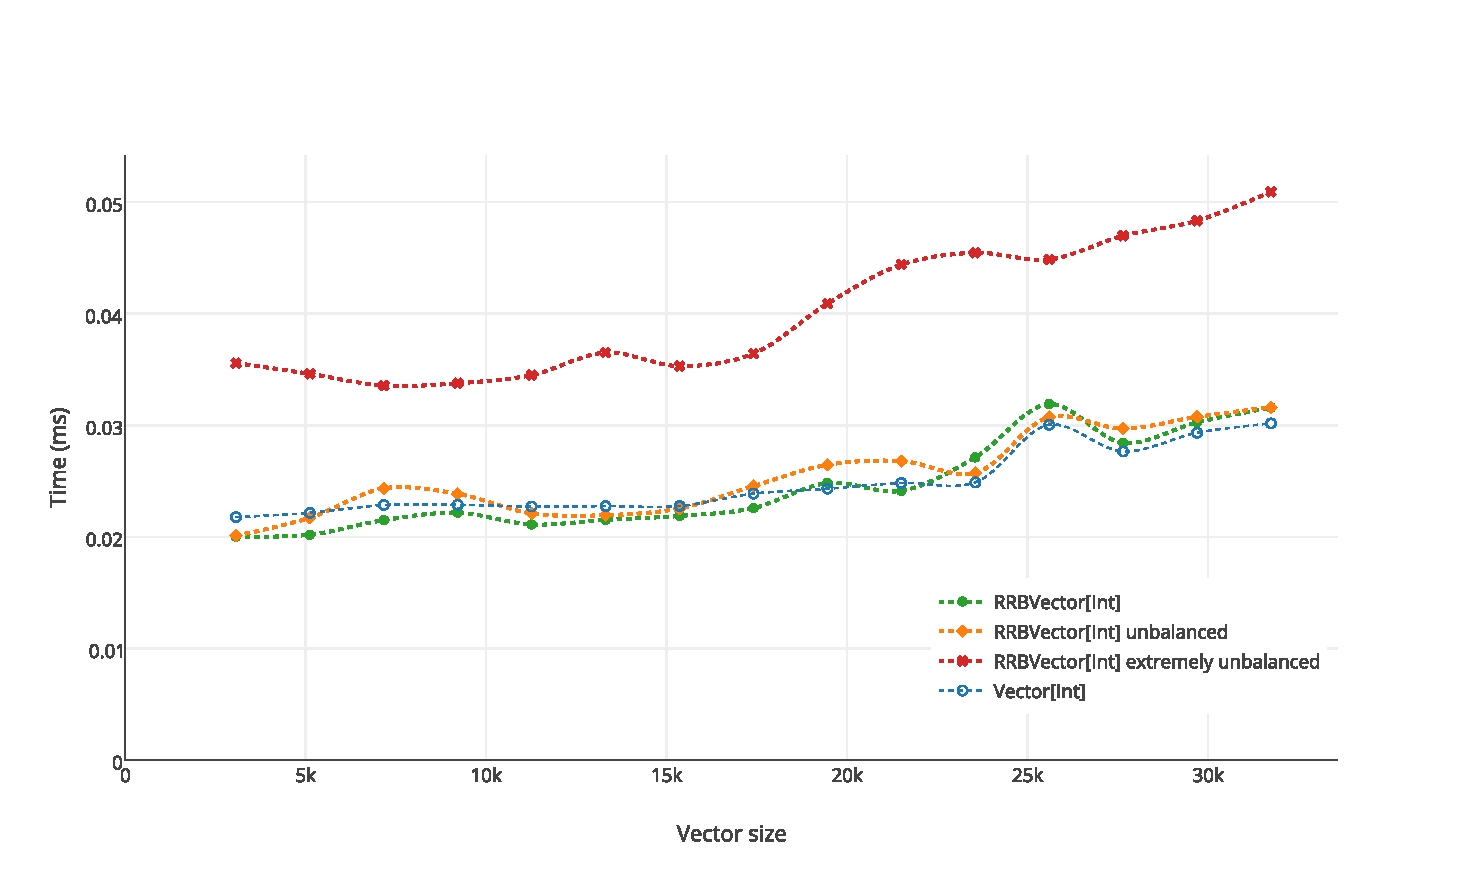
\includegraphics[width=\textwidth]{Benchmarks/Append_3.pdf}
  \label{Append3Benchmarks}
  \caption{Time to execute 256 append operations. This shows the amortized cost of the append operation.}
\end{figure}

\begin{figure}[h!]
  \centering
  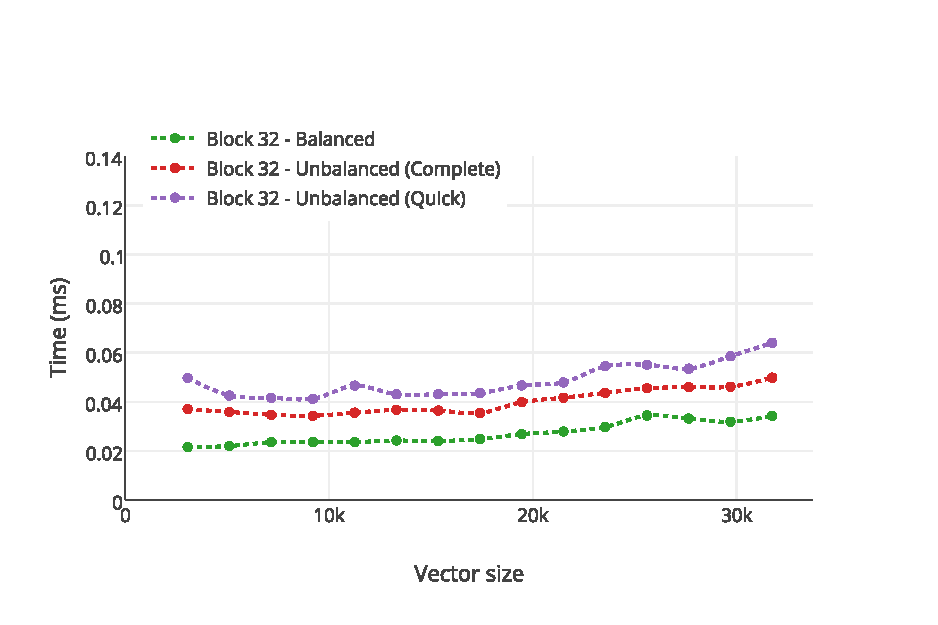
\includegraphics[width=0.49\textwidth]{Benchmarks/Append_blocks_32.pdf}
  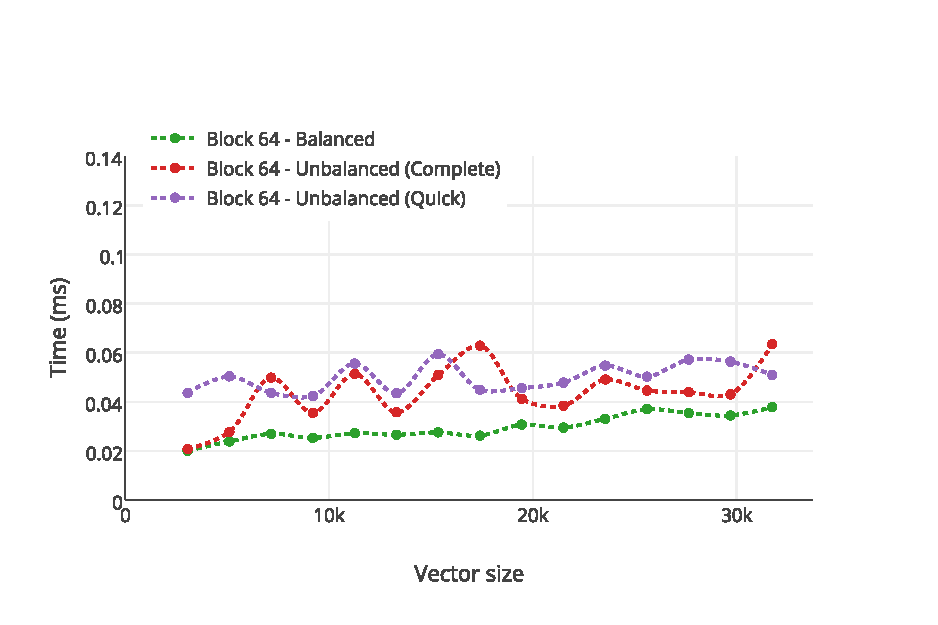
\includegraphics[width=0.49\textwidth]{Benchmarks/Append_blocks_64.pdf}
  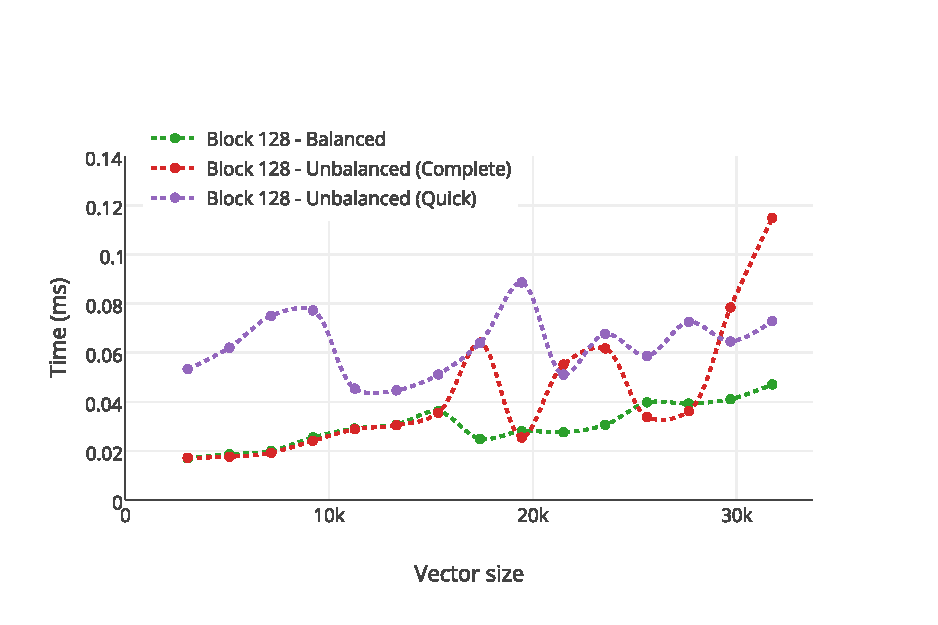
\includegraphics[width=0.49\textwidth]{Benchmarks/Append_blocks_128.pdf}
  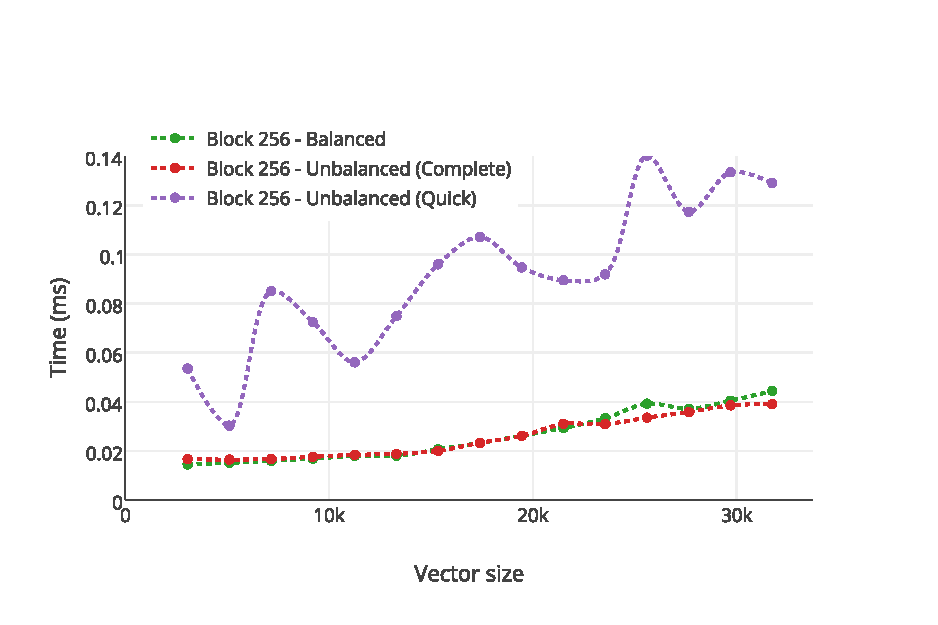
\includegraphics[width=0.49\textwidth]{Benchmarks/Append_blocks_256.pdf}
  \label{IterationBlocksBenchmarks}
  \caption{Time to execute 256 append operations. This shows the amortized cost of the append operation. Comparing performances for different block sizes and different implementation of the concatenation inner branch rebalancing (Complete/Quick).}
\end{figure}

%-----------------------------------
%	SUBSECTION Prepend
%-----------------------------------
\subsection{Prepend}
% describe the benchmark function
% compare expectation with results
% explain the upper bound
% explain apparently incoherent results

\begin{figure}[h!]
  \centering
  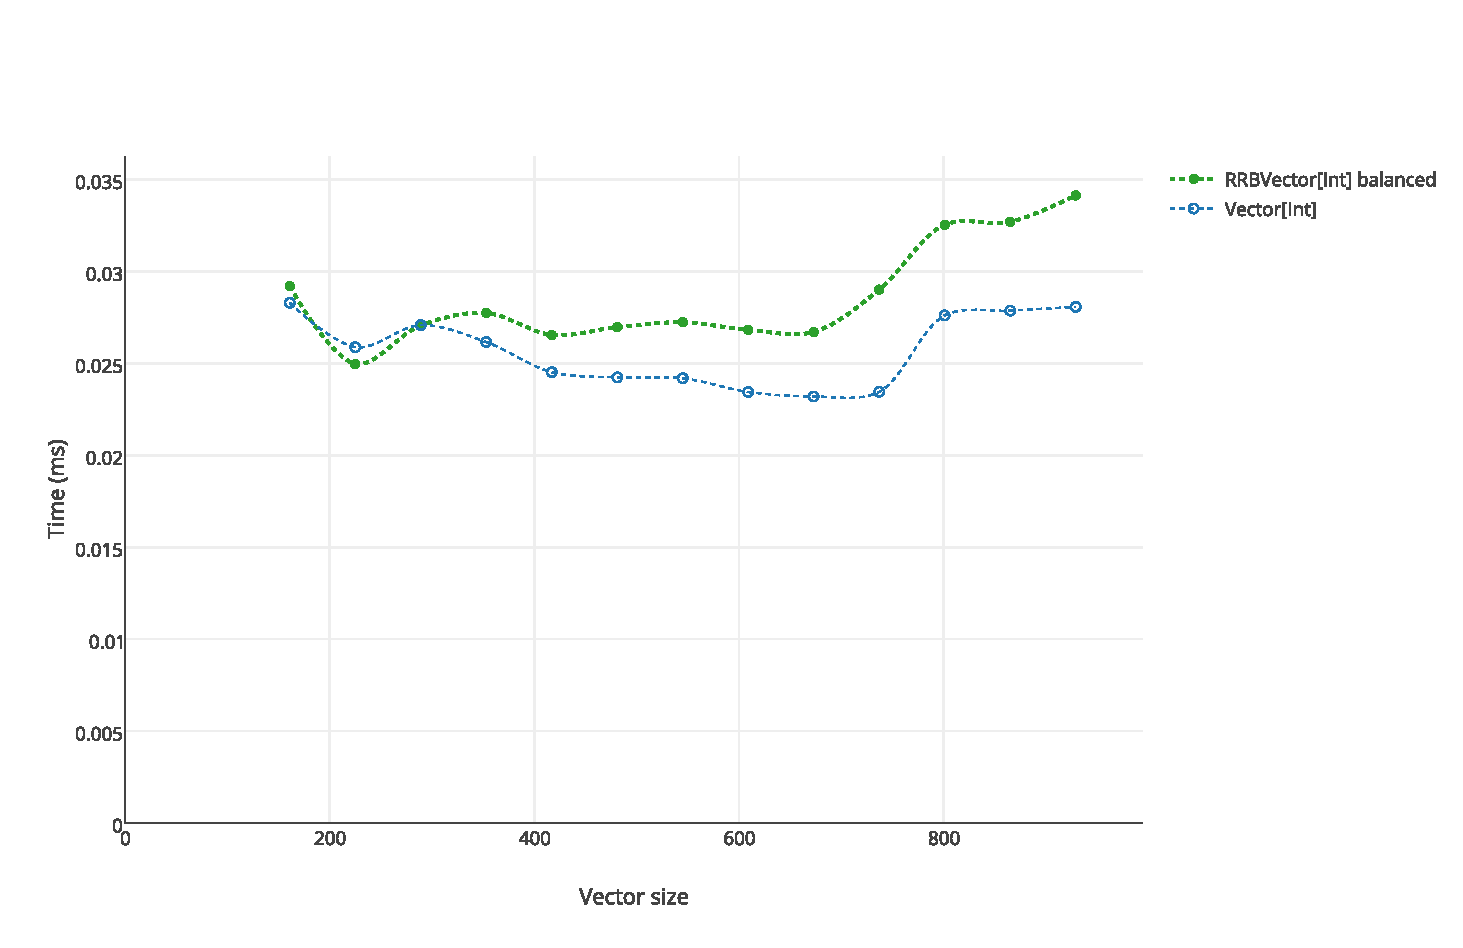
\includegraphics[width=\textwidth]{Benchmarks/Prepend_2.pdf}
  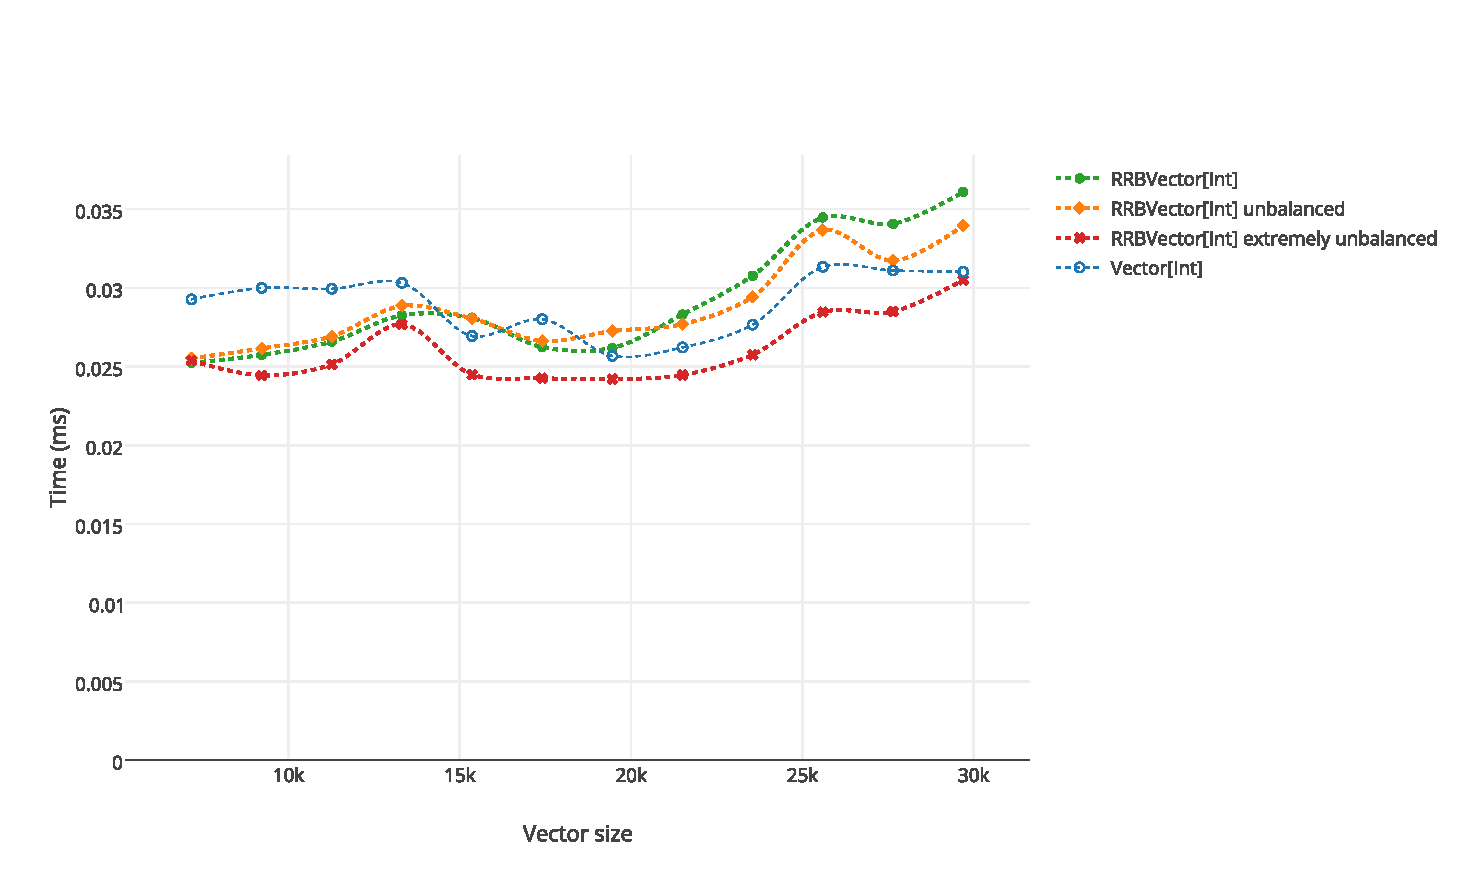
\includegraphics[width=\textwidth]{Benchmarks/Prepend_3.pdf}
  \label{PrependBenchmarks}
  \caption{Time to execute 256 prepend operations. This shows the amortized cost of the prepend operation.}
\end{figure}

\begin{figure}[h!]
  \centering
  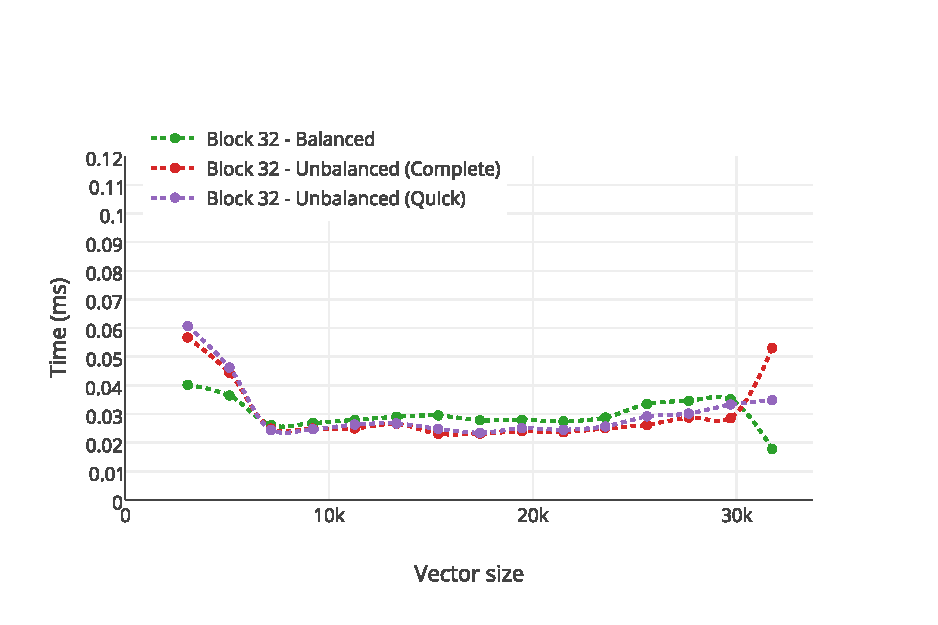
\includegraphics[width=0.49\textwidth]{Benchmarks/Prepend_blocks_32.pdf}
  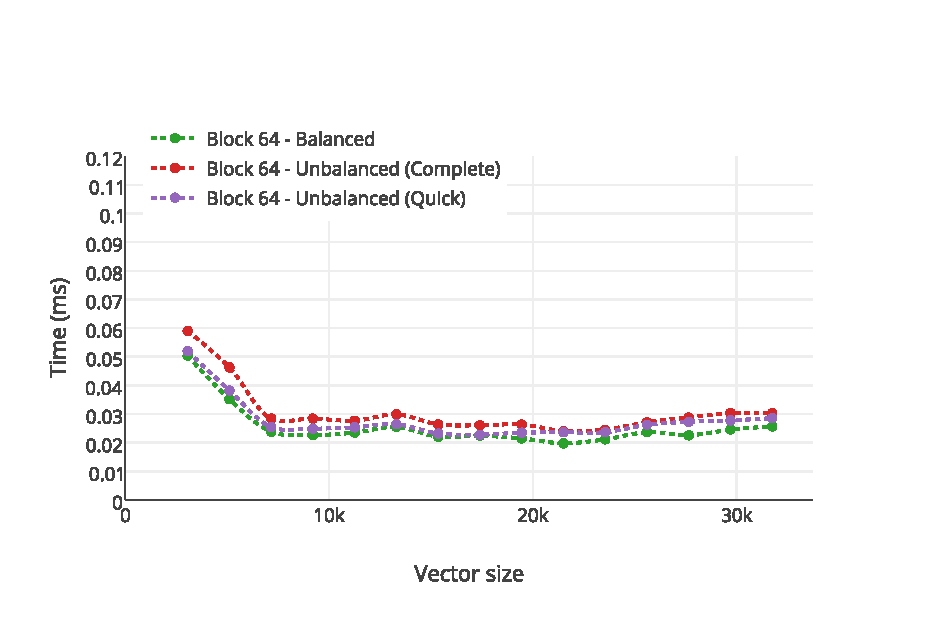
\includegraphics[width=0.49\textwidth]{Benchmarks/Prepend_blocks_64.pdf}
  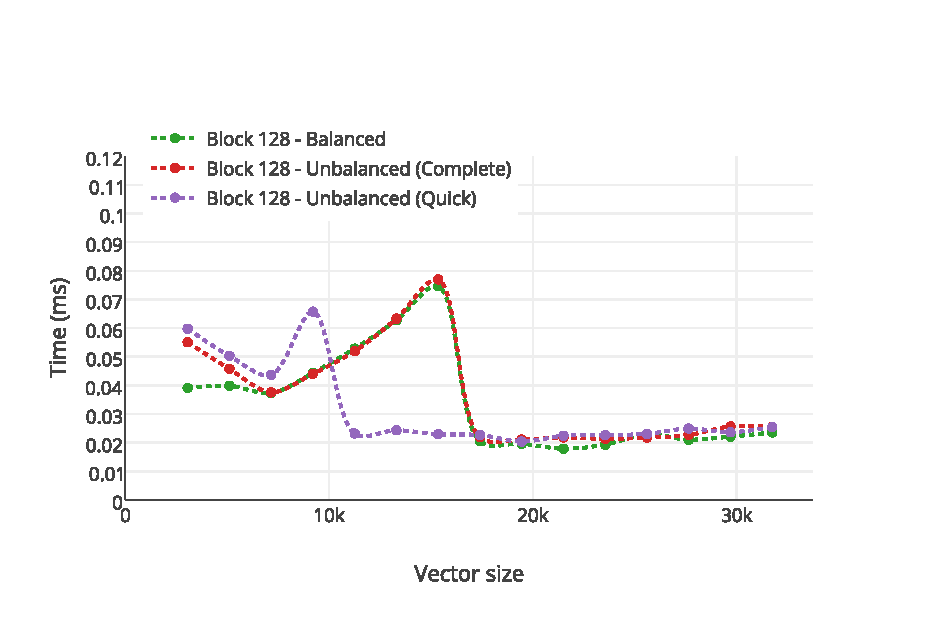
\includegraphics[width=0.49\textwidth]{Benchmarks/Prepend_blocks_128.pdf}
  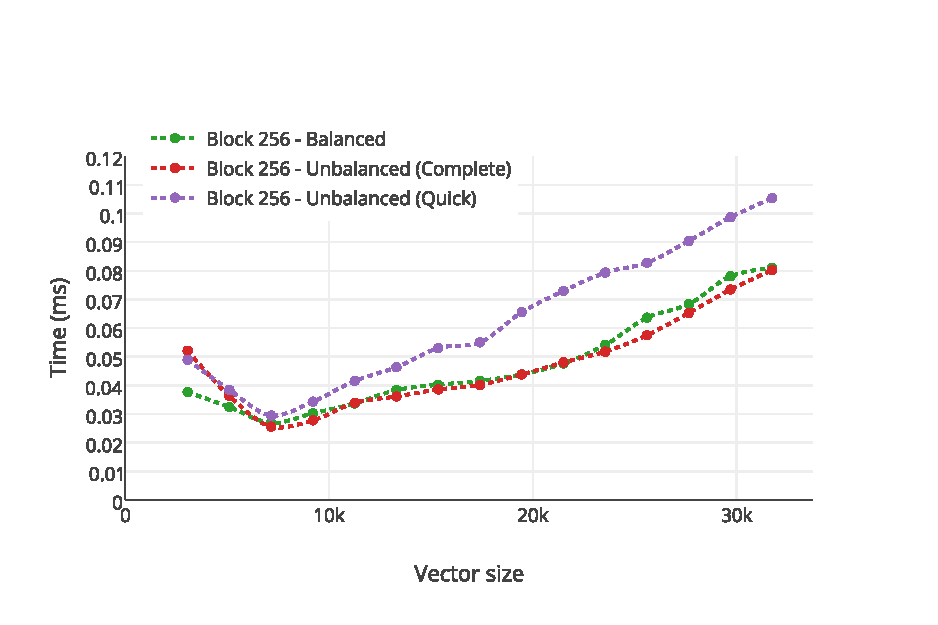
\includegraphics[width=0.49\textwidth]{Benchmarks/Prepend_blocks_256.pdf}
  \label{PrependBenchmarks}
  \caption{Time to execute 256 prepend operations. This shows the amortized cost of the append operation. Comparing performances for different block sizes and different implementation of the concatenation inner branch rebalancing (Complete/Quick).}
\end{figure}


%-----------------------------------
%	SUBSECTION Splits
%-----------------------------------
\subsection{Splits}
% describe the benchmark function
% compare expectation with results
% explain the upper bound
% explain apparently incoherent results

\begin{figure}[h!]
  \centering
  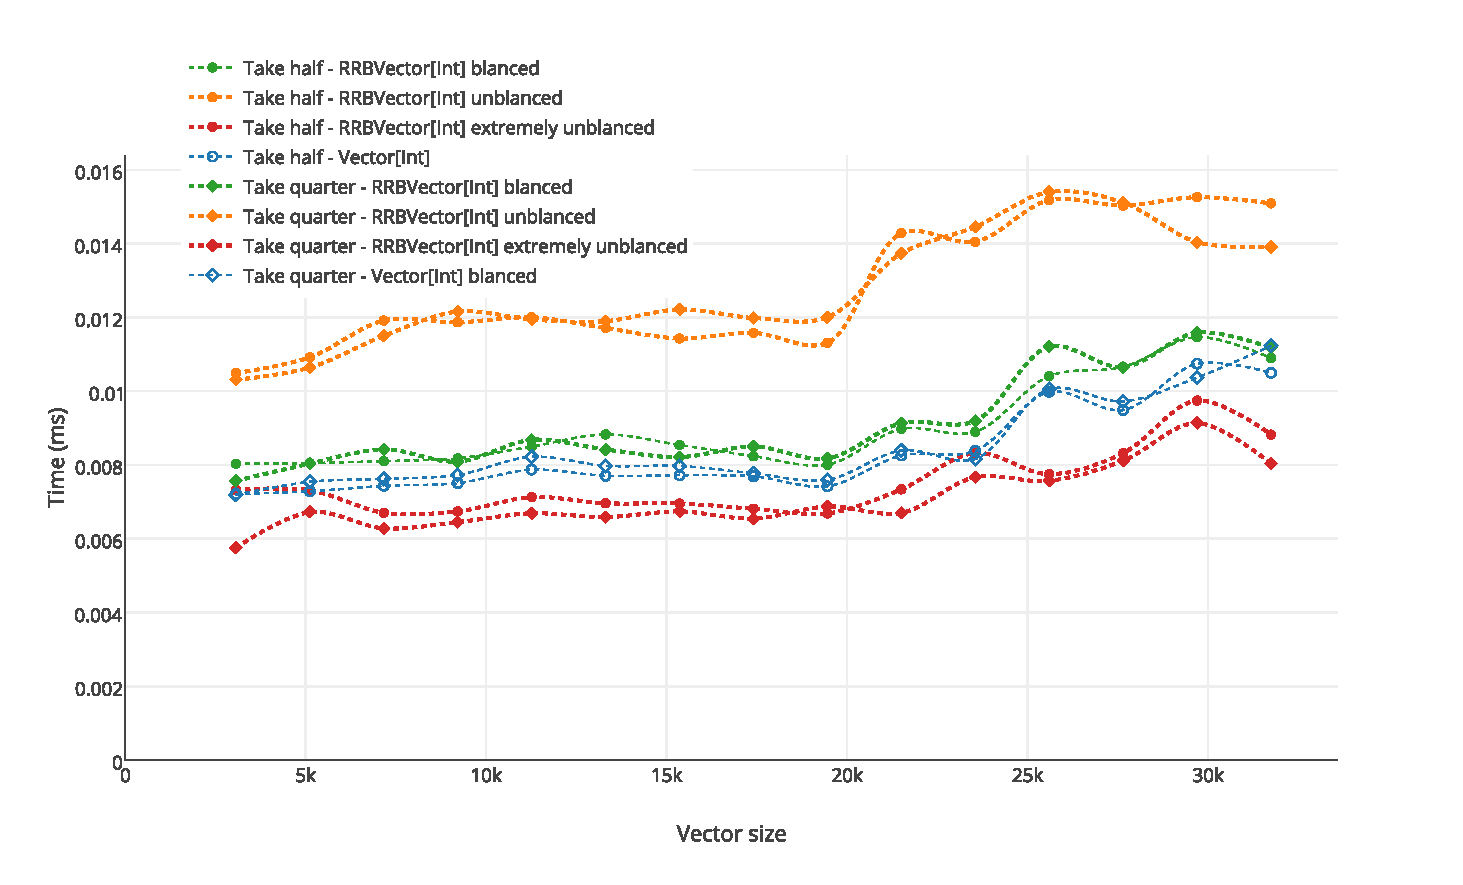
\includegraphics[width=\textwidth]{Benchmarks/Split_take_3.pdf}
  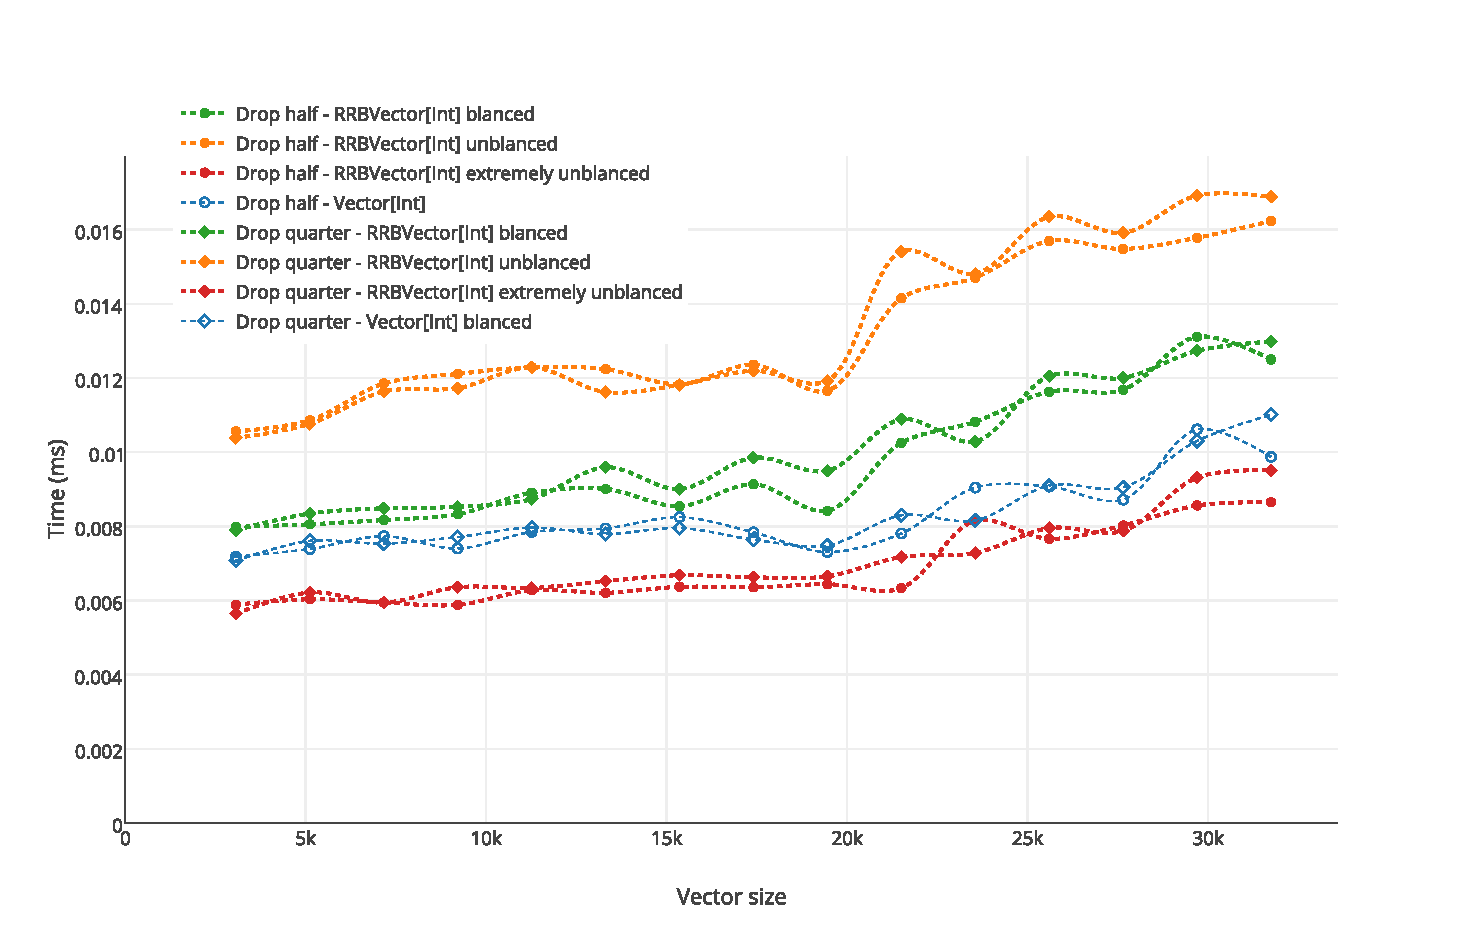
\includegraphics[width=\textwidth]{Benchmarks/Split_drop_3.pdf}
  \label{SplitsBenchmarks}
  \caption{Execution time of take and drop.}
\end{figure}


%-----------------------------------
%	SUBSECTION Iterator
%-----------------------------------
\subsection{Iterator}
% describe the benchmark function
% compare expectation with results
% explain the upper bound
% explain apparently incoherent results: iteration of sightly unbalanced vector is faster

\begin{figure}[h!]
  \centering
  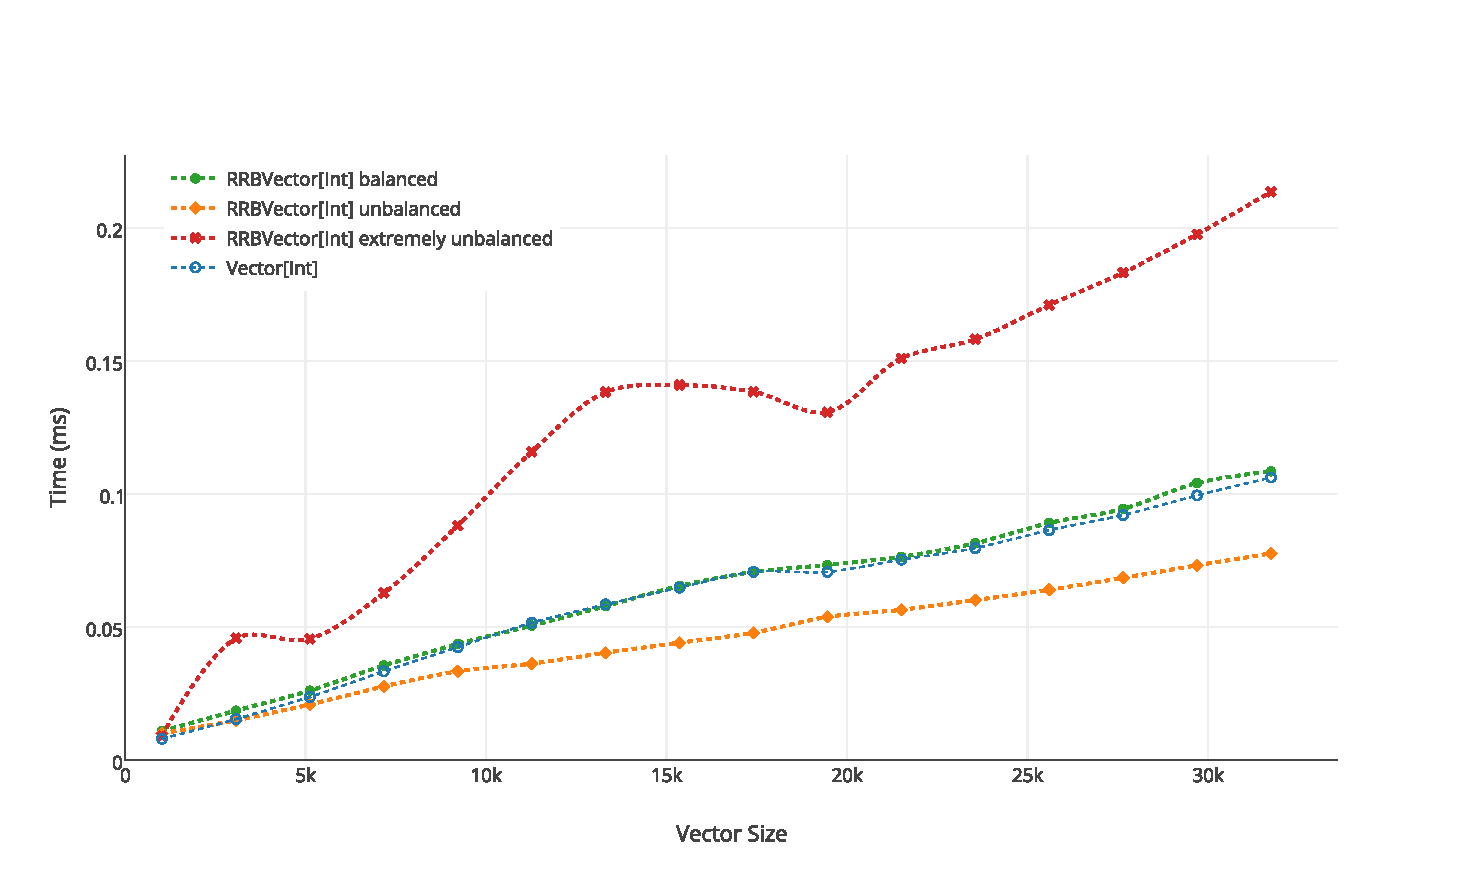
\includegraphics[width=\textwidth]{Benchmarks/Iteration_3.pdf}
  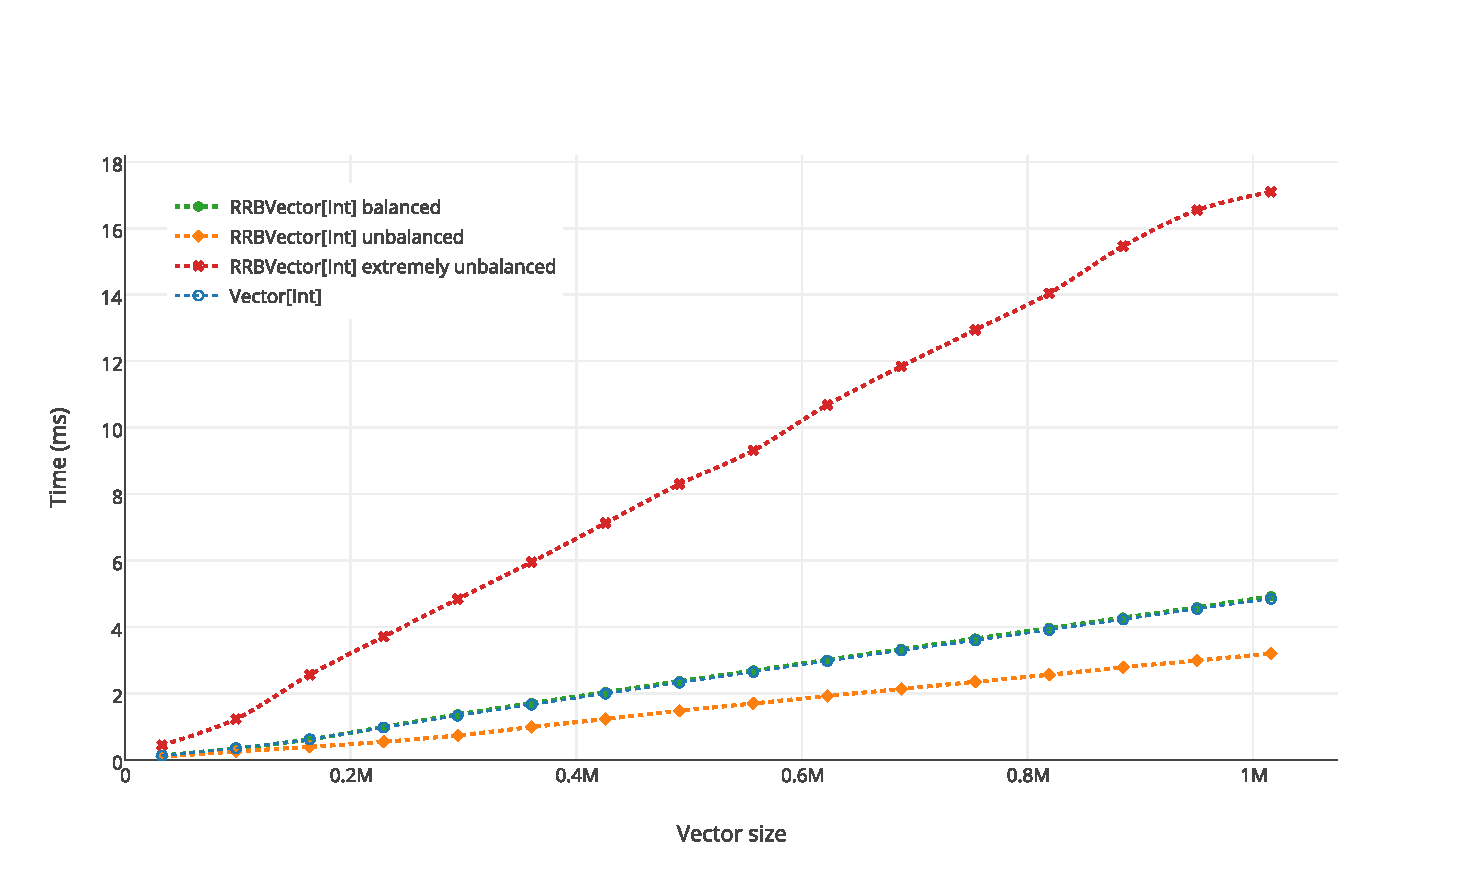
\includegraphics[width=\textwidth]{Benchmarks/Iteration_4.pdf}
  \label{IterationBenchmarks}
  \caption{Excecution time to iterate through all the elements of the vector.}
\end{figure}

\begin{figure}[h!]
  \centering
  \label{IterationBlocksBenchmarks}
  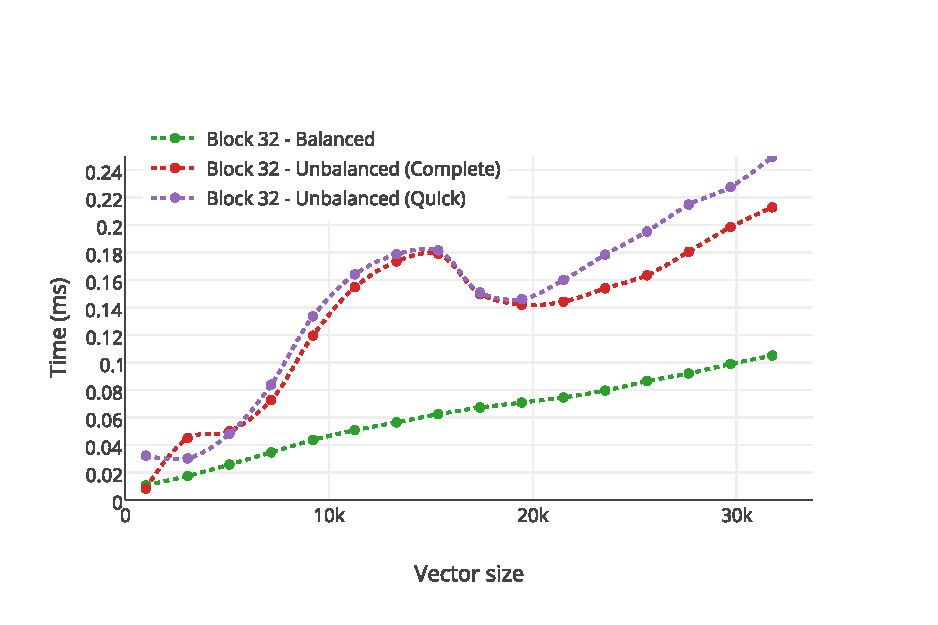
\includegraphics[width=0.49\textwidth]{Benchmarks/Iteration_blocks_32.pdf}
  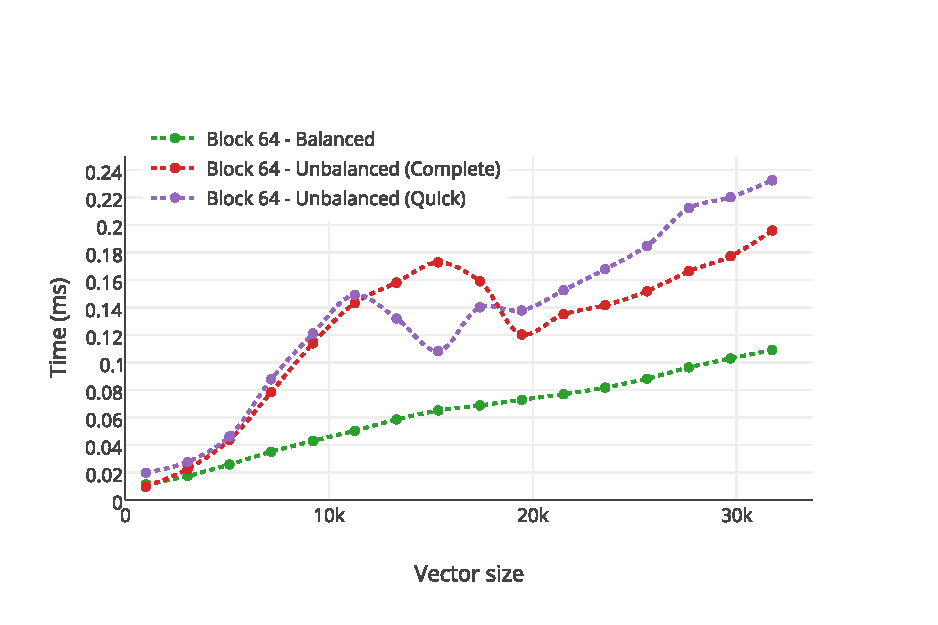
\includegraphics[width=0.49\textwidth]{Benchmarks/Iteration_blocks_64.pdf}
  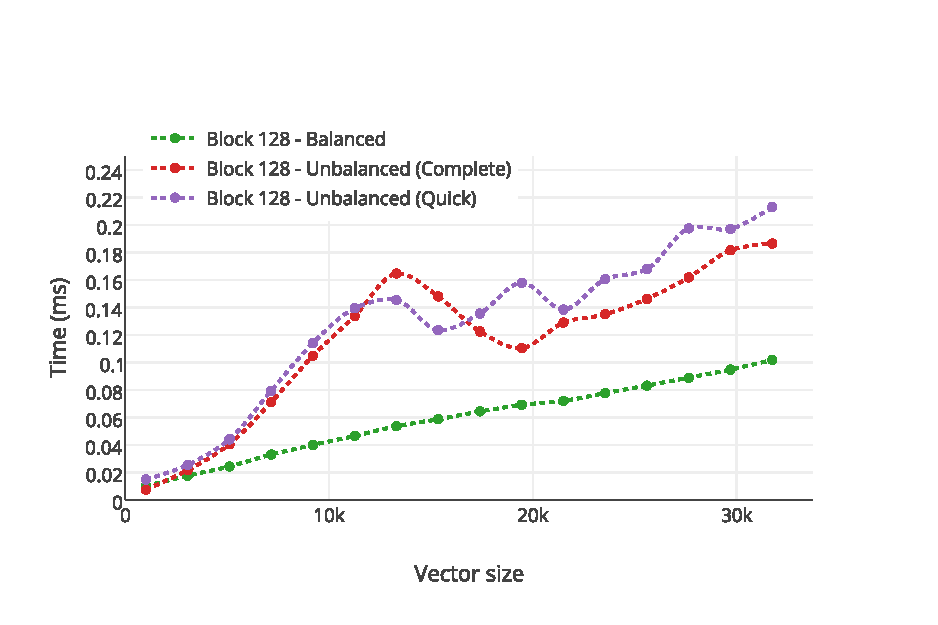
\includegraphics[width=0.49\textwidth]{Benchmarks/Iteration_blocks_128.pdf}
  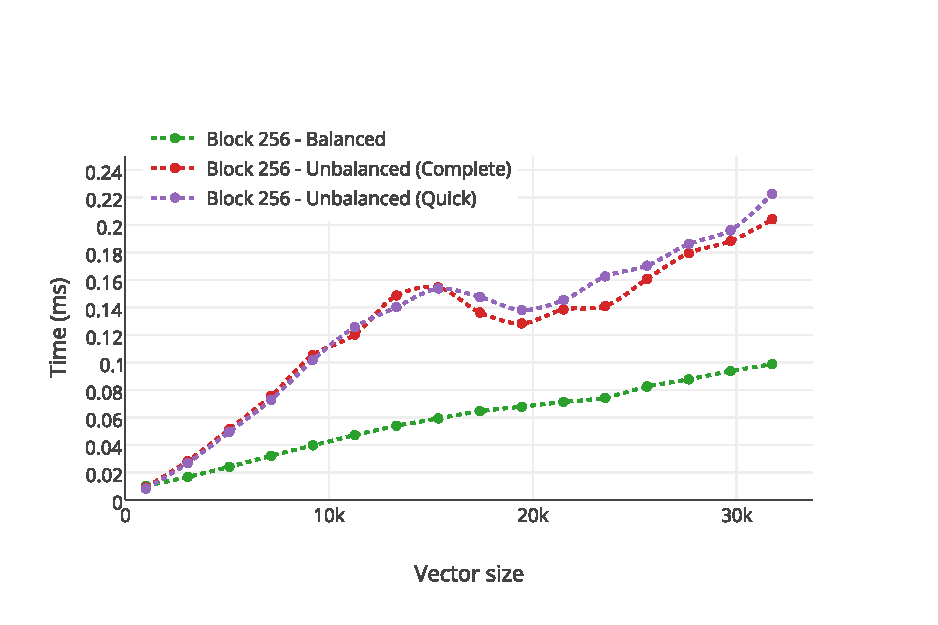
\includegraphics[width=0.49\textwidth]{Benchmarks/Iteration_blocks_256.pdf}
  \caption{Excecution time to iterate through all the elements of the vector. Comparing performances for different block sizes and different implementation of the concatenation inner branch rebalancing (Complete/Quick).}
\end{figure}

%-----------------------------------
%	SUBSECTION Builder
%-----------------------------------
\subsection{Builder}
% describe the benchmark function
% compare expectation with results
% explain the upper bound
% explain apparently incoherent results

\begin{figure}[h!]
  \centering
  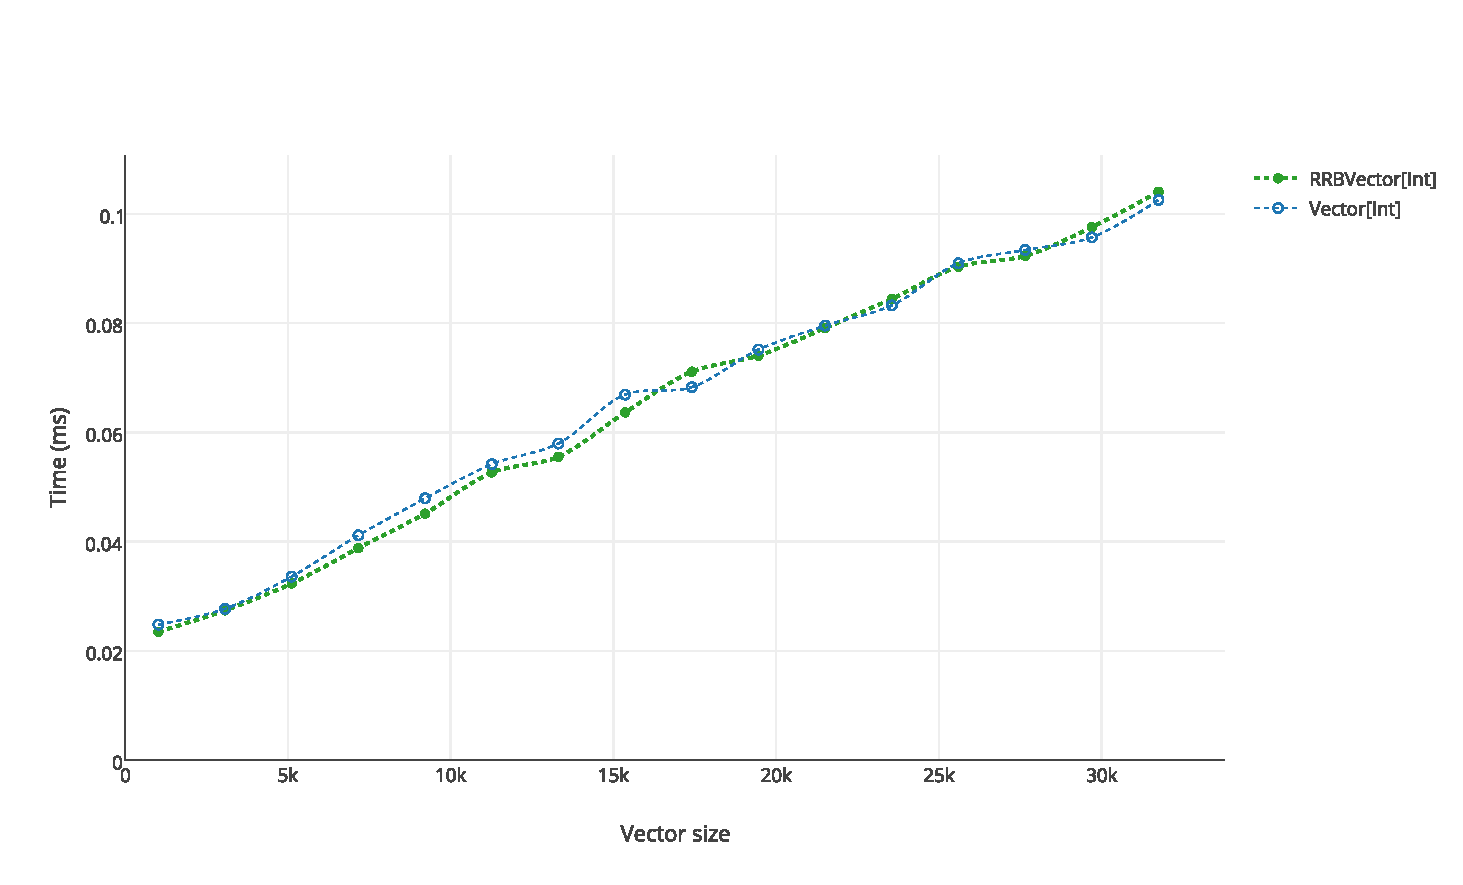
\includegraphics[width=\textwidth]{Benchmarks/Builder_3.pdf}
  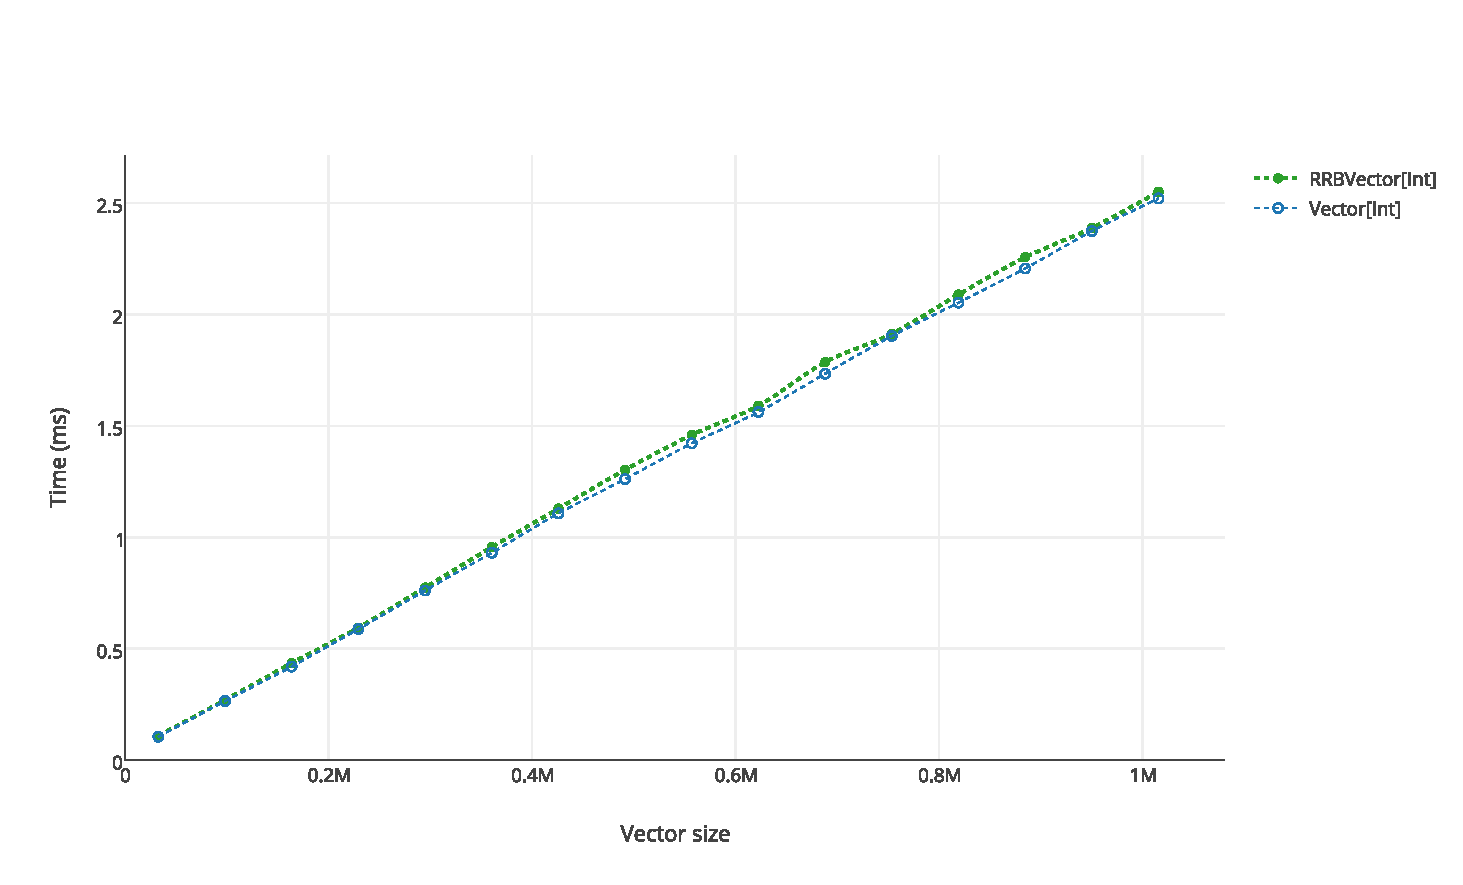
\includegraphics[width=\textwidth]{Benchmarks/Builder_4.pdf}
  \label{BuilderBenchmarks}
  \caption{Execution time to build a vector of a given size.}
\end{figure}

\begin{figure}[h!]
  \centering
  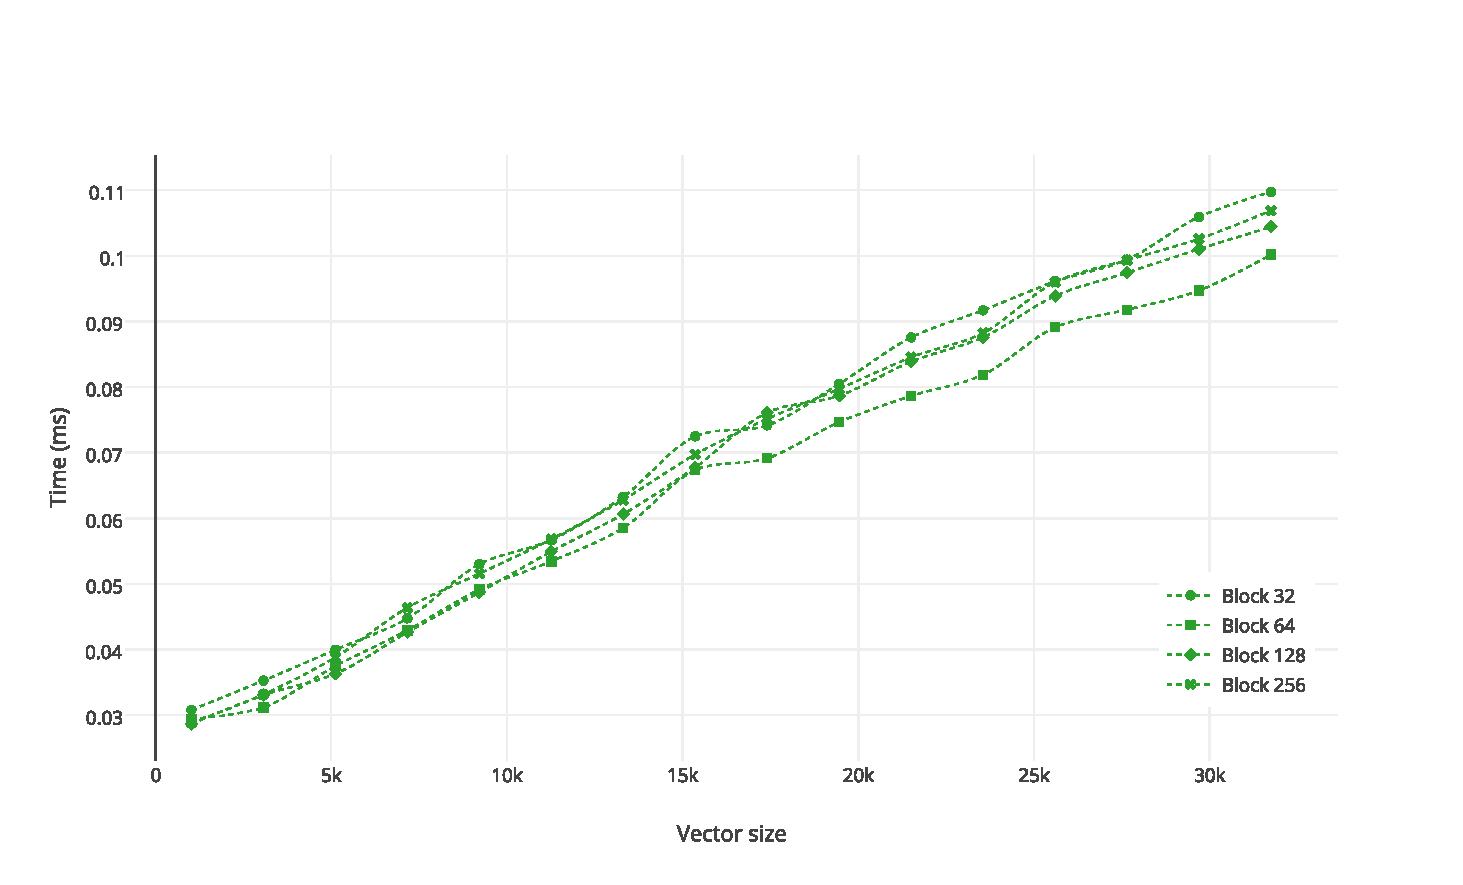
\includegraphics[width=\textwidth]{Benchmarks/Builder_blocks.pdf}
  \label{BuilderBlocksBenchmarks}
  \caption{Execution time to build a vector of a given size. Comparing performances for different block sizes.}
\end{figure}

%-----------------------------------
%	SUBSECTION Parallel split-combine
%-----------------------------------
\subsection{Parallel split-combine}
% describe the benchmark function
% compare expectation with results
% explain the upper bound
% explain apparently incoherent results

\begin{figure}[h!]
  \centering
  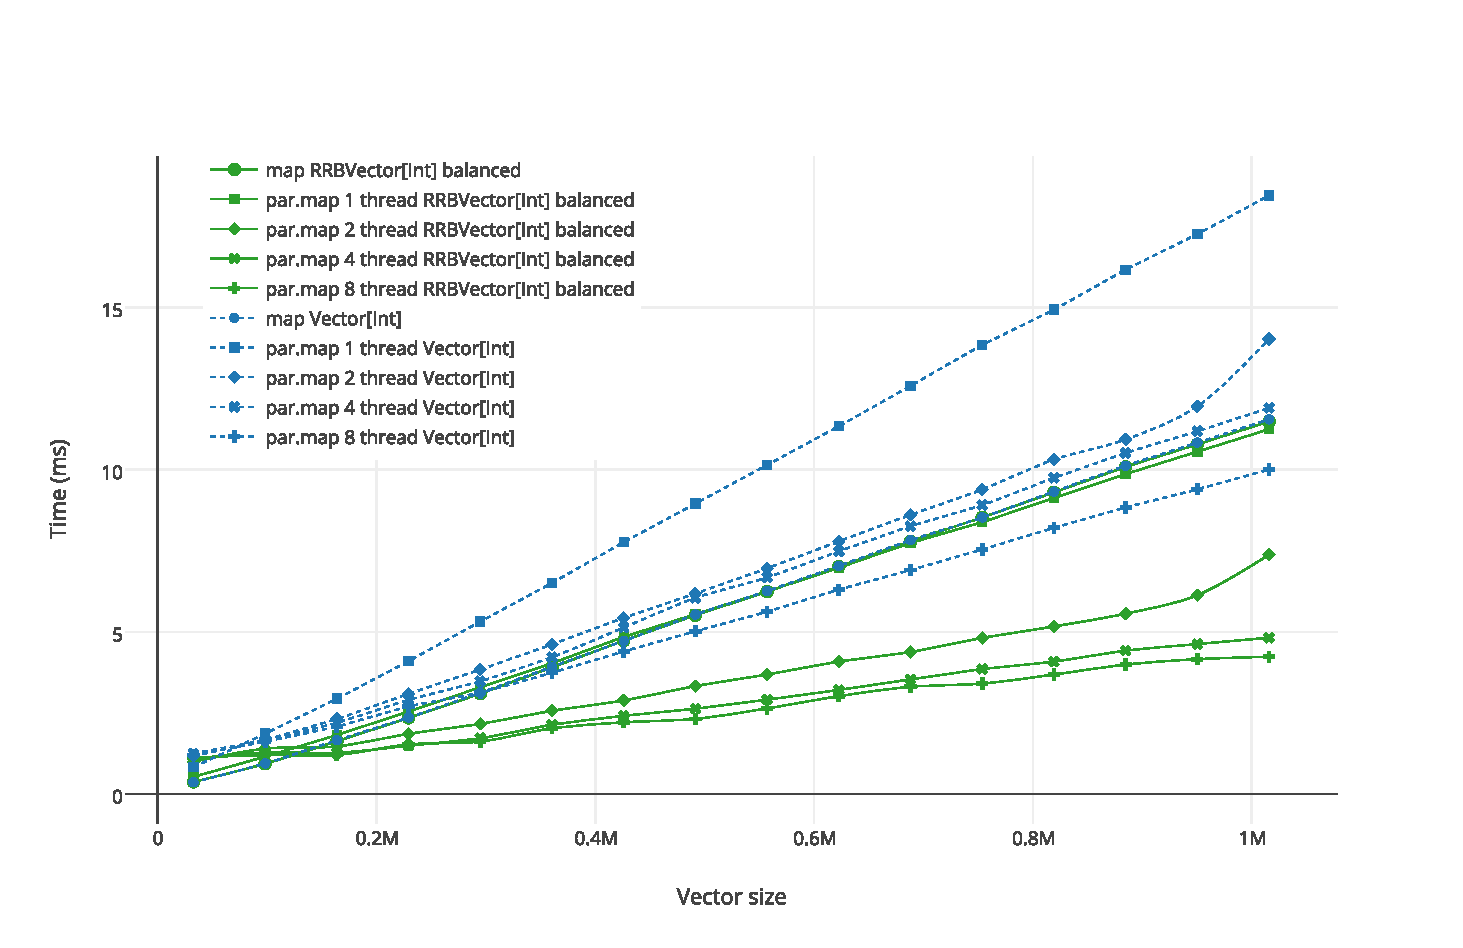
\includegraphics[width=\textwidth]{Benchmarks/Parmap_balanced.pdf}
  \label{ParallelBenchmarks}
  \caption{Benchmark on map and parallel map using the function (\textsc{x=>x}) to show the difference time used in the framework. This time represents the time spent in the splitters and combiners of the parallel collection (iterator and builder for the sequential version).}
\end{figure}

\begin{figure}[h!]
  \centering
  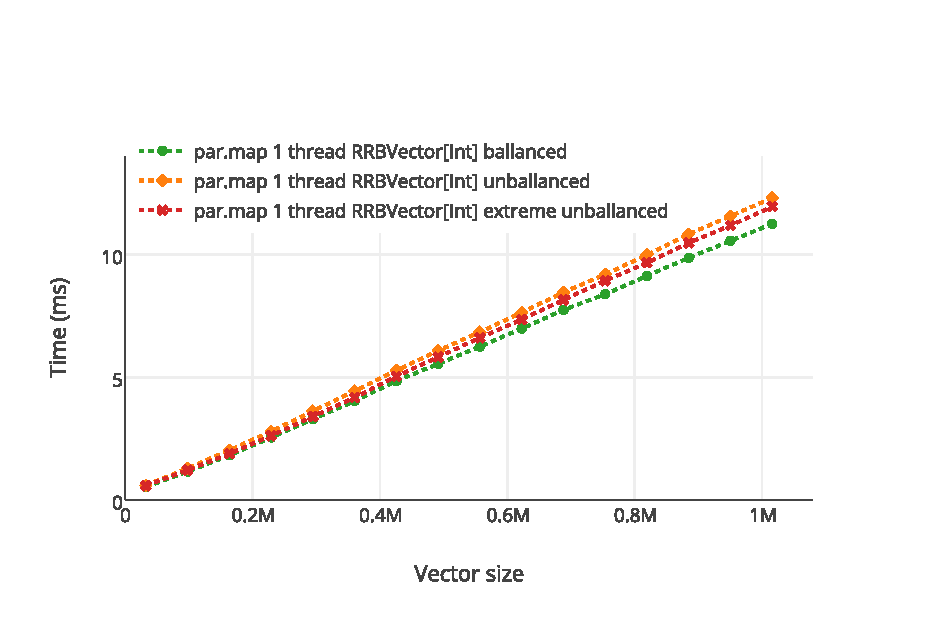
\includegraphics[width=0.49\textwidth]{Benchmarks/parmap_unbalanced_1.pdf}
  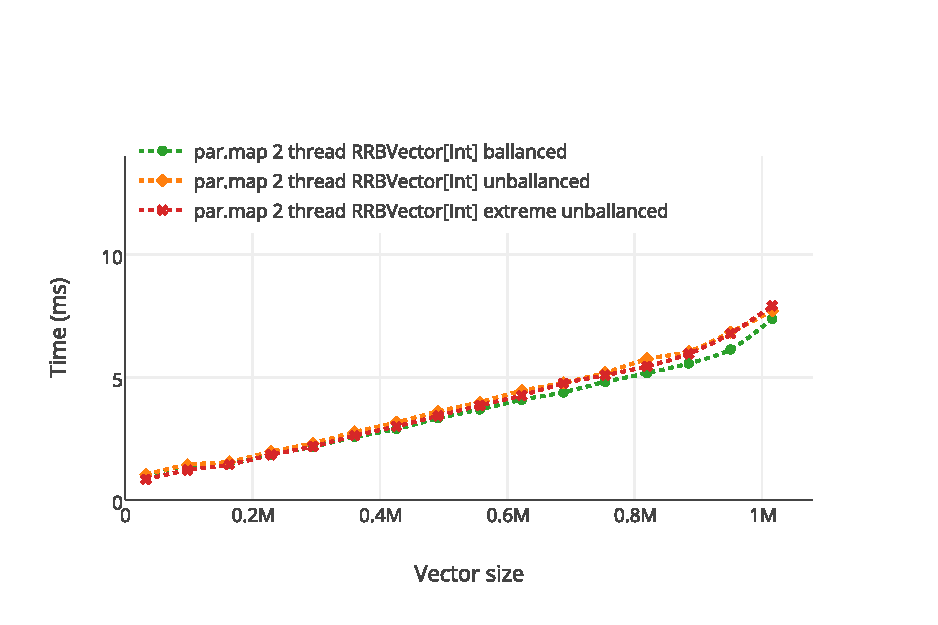
\includegraphics[width=0.49\textwidth]{Benchmarks/parmap_unbalanced_2.pdf}
  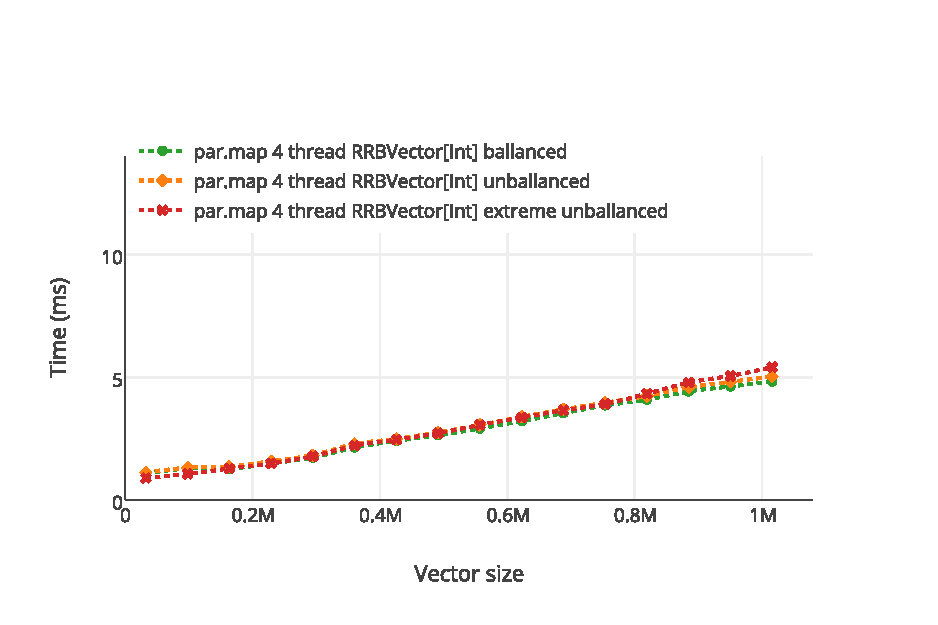
\includegraphics[width=0.49\textwidth]{Benchmarks/parmap_unbalanced_4.pdf}
  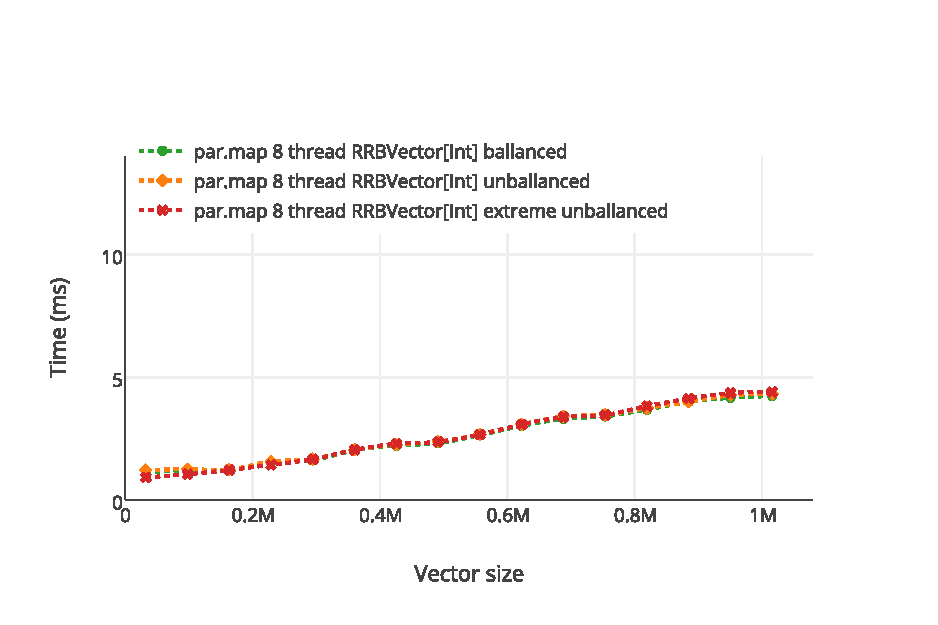
\includegraphics[width=0.49\textwidth]{Benchmarks/parmap_unbalanced_8.pdf}
  \label{ParallelUnbalancedBenchmarks}
  \caption{Benchmark on map and parallel map using the function (\textsc{x=>x}) to show the difference time used in the framework. This time represents the time spent in the splitters and combiners of the parallel collection.}
\end{figure}


%-----------------------------------
%	SUBSECTION Memory footprint
%-----------------------------------

\subsection{Memory footprint}
% describe the benchmark function
% compare expectation with results
% explain the upper bound
% explain apparently incoherent results

\begin{figure}[h!]
  \centering
  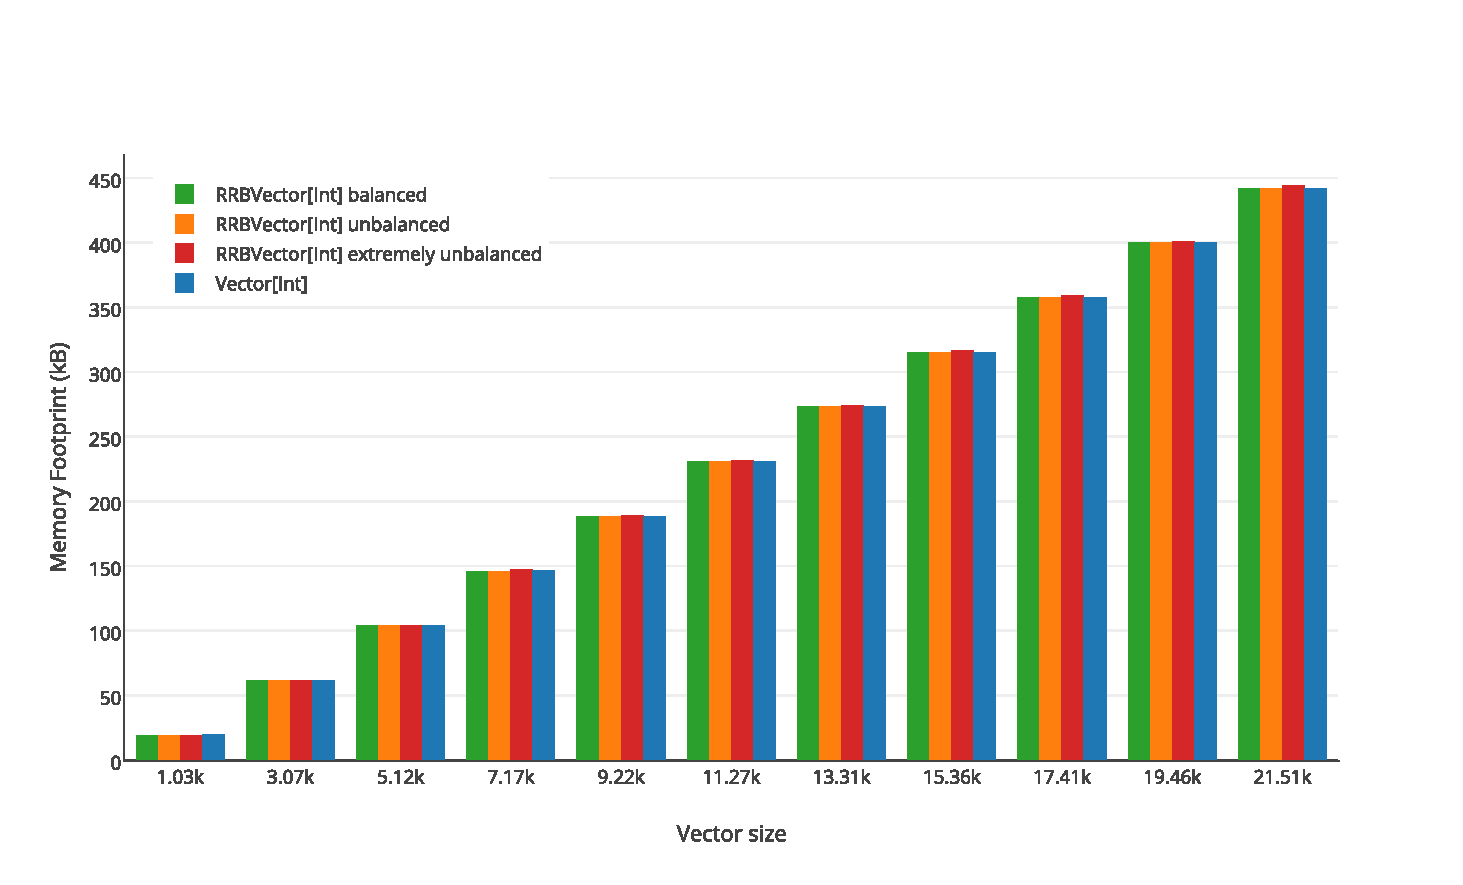
\includegraphics[width=\textwidth]{Benchmarks/Memory_3.pdf}
  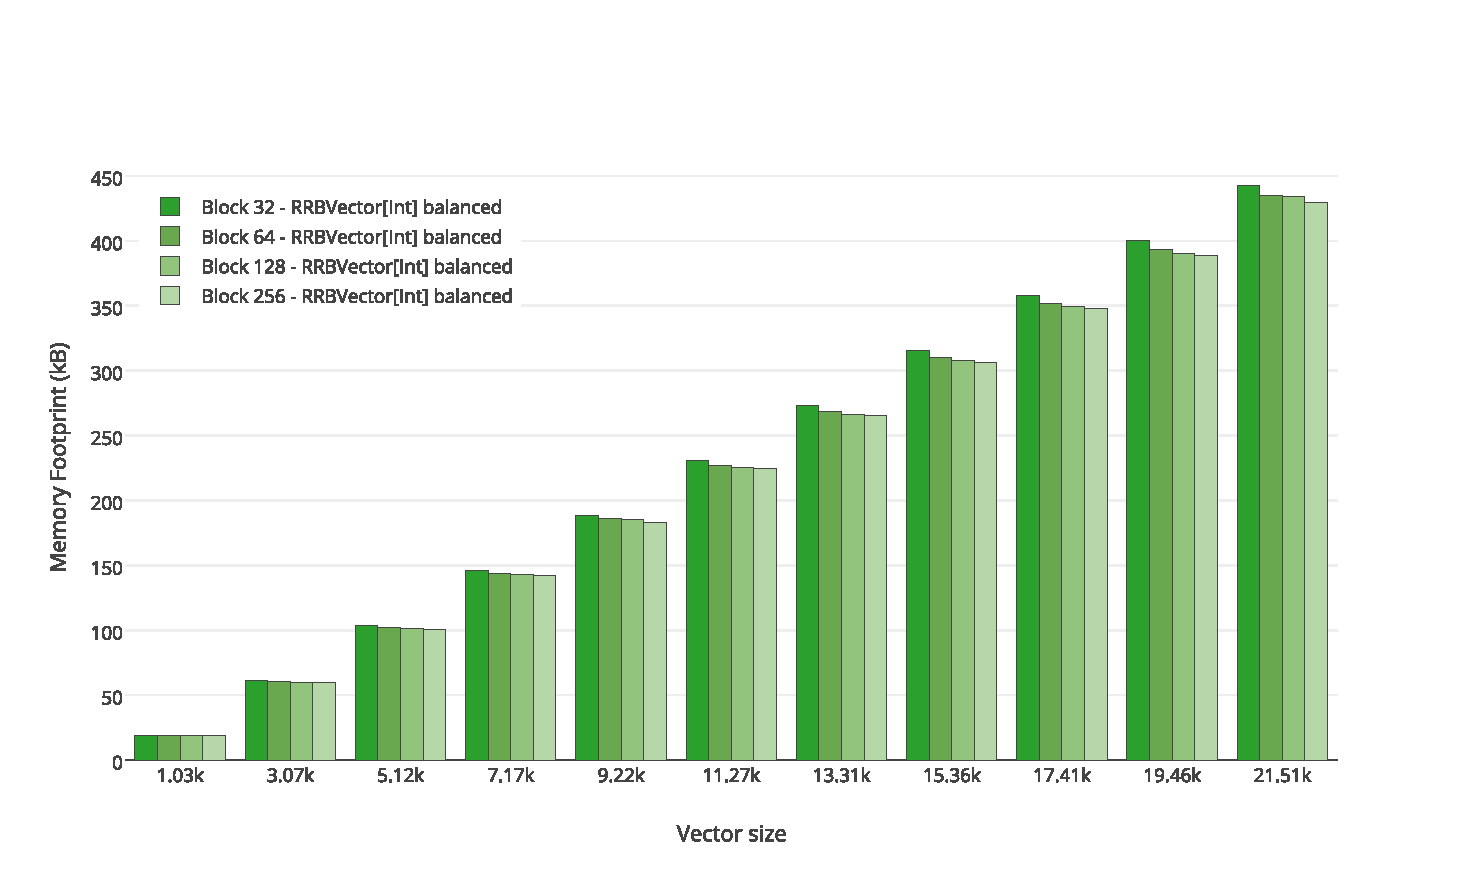
\includegraphics[width=\textwidth]{Benchmarks/Memory_blocks.pdf}
  \label{MemoryFootprints}
  \caption{Memory Footprint}
\end{figure}



